% !TeX spellcheck = en_US

\section{Filter Comparison}

\subsection{Architectural differences}
\label{sec:filter_comp_subsec:architectural_diff}
The main difference of each pack of filters is the architecture itself.
Using a standard multiplier, the filter coefficients are multiplied with the input samples using multipliers. The output is obtained by summing the products of the coefficients and input samples. This architecture is straightforward and produces accurate results but can be resource-intensive in terms of hardware implementation.

The second implementation is by using factored CSD. This is a technique used to reduce the number of partial products required for multiplication by decomposing the coefficients into a sum of powers of two. This architecture employs a combination of shifters and adders to implement the multiplication operation. The output is obtained by accumulating the partial products. Factored CSD reduces hardware complexity and power consumption compared to the multiplier architecture, but it may introduce some additional round-off errors due to approximation.

The last architecture used in this project is called Distributed Arithmetic (\emph{DA}).
Distributed arithmetic is another technique for efficient multiplication using look-up tables (LUTs). In this architecture, the filter coefficients are precomputed and stored in a LUT. The input samples are used as indices to retrieve the corresponding precomputed values from the LUT. These values are then summed to obtain the filter output. Distributed arithmetic offers advantages in terms of reduced hardware complexity and power consumption but can introduce quantization errors due to the finite precision of the LUT.

So, when comparing these architectures, we can expect the multiplier architecture to provide the most accurate results but at the cost of increased hardware complexity and power consumption.
The factored CSD and distributed arithmetic architectures offer trade-offs by reducing hardware requirements and power consumption while introducing minor approximations that result in slight differences in the output.

\subsection{Minimum Order filter}
Beginning with the minimum order one, overall utilization is fairly low due to the low number of coefficients used. From MATLAB, the minimum coeff.\hspace{-3pt} number that was able to produce an \verb|FIR| filter of those specifications was \textbf{3}.
Creating a filter with such low number of coefficients does not have a great filtering capability as can be seen from figure~\ref{fig:min_order_filt}.

\begin{wrapfigure}{R}{0.25\textwidth}
	\centering
	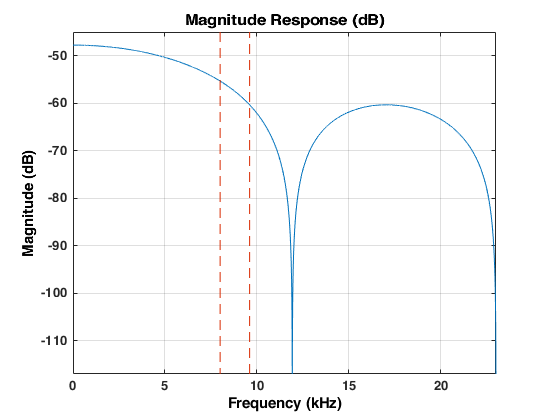
\includegraphics[width=0.25\textwidth]{../Images/FIR_min_Order/min_order_filt.png}
	\caption{Magnitude response of the FIR filter with minimum number of coefficients.}
	\label{fig:min_order_filt}
\end{wrapfigure}

Increasing pipeline stages from one to two, theoretically, increases operations per cycle but it didn't have the same impact on execution time.
From figure~\ref{fig:exec_time_min_32b}, we can see that execution time of 1-stage pipeline is faster than 2-stage pipeline by a significant margin. This decrease in execution time is due to several overheads from the second pipeline stage but the increase of those stages can increase efficiency by dropping operating frequency while doing the same amount of computations in the same time (\textit{because of the reduced slack}).

%\begin{figure}[htbp]
%	\centering
%	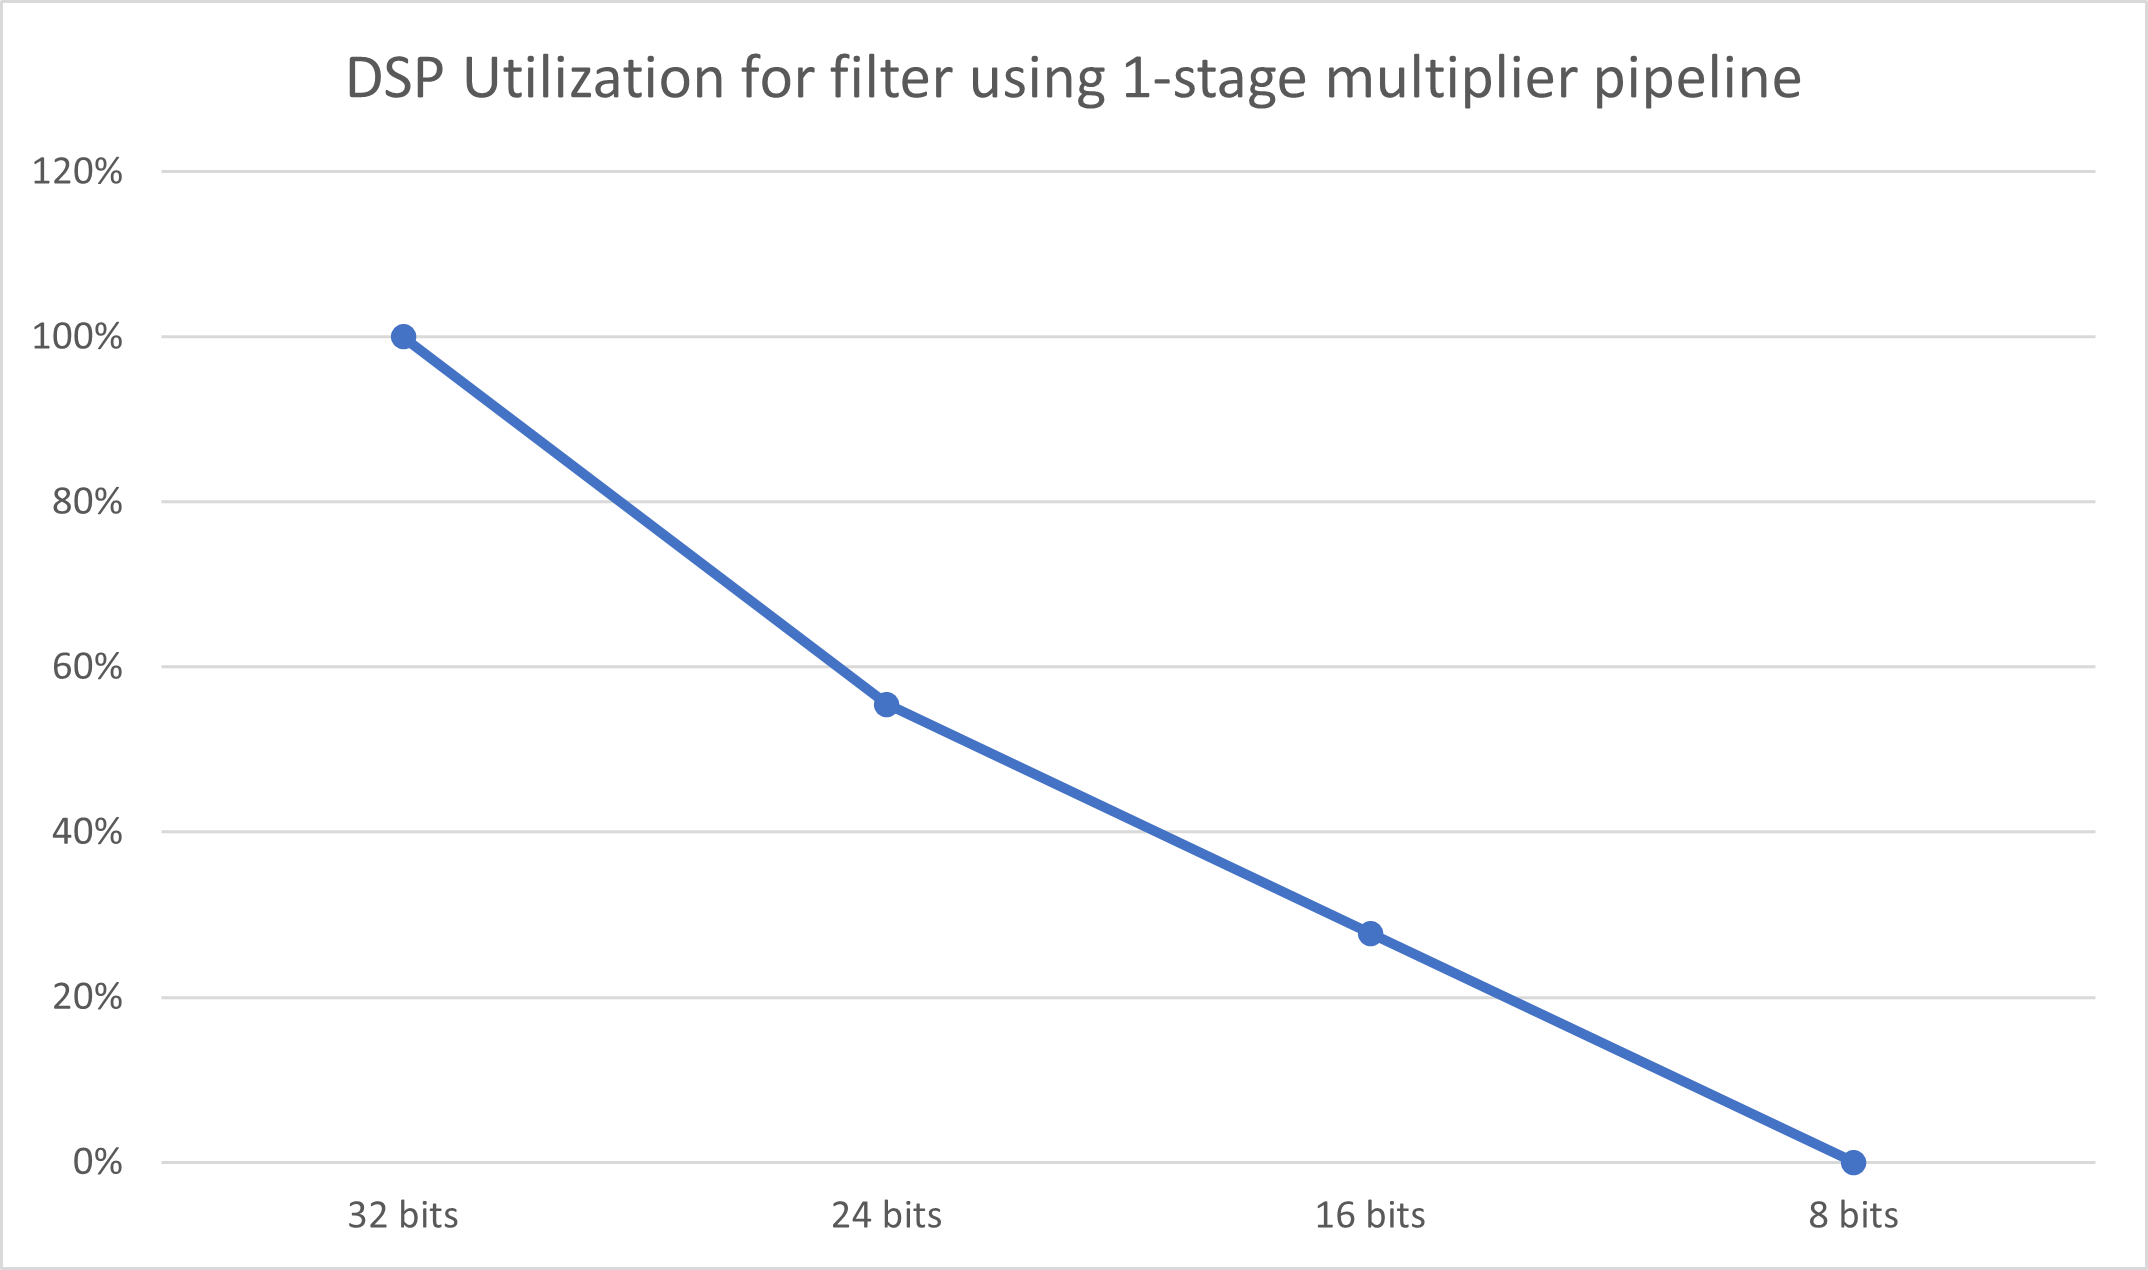
\includegraphics[width=0.45\textwidth]{../Images/FIR_min_Order/multiplier_1_pipeline/dsp_util.png}
%	\caption{DSP utilization for min. order filter (\textit{multiplier 1-stage}) using different bits}
%	\label{fig:fir_min_dsp_util}
%\end{figure}
%
%\begin{table}[htbp]
%\centering
%\begin{tblr}{|c|c|}
%	\hline
%	Architecture & Time \\
%	\hline
%	{Multiplier 1-stage pipeline} & 35140 ns\\
%	\hline
%	{Multiplier 2-stage pipeline} & 35160 ns\\
%	\hline
%\end{tblr}
%\caption{Time for different multiplier pipeline stages using 32 bit floating point arithmetic.}
%\label{table:multiplier_stages_time}
%\end{table}

Knowing the latency of each architecture, we can calculate the overall execution time for a specific sample set. MATLAB's sample set consists of $3499$ samples. So, using the following formula, we can calculate each architecture's execution time.
\begin{small}
\begin{equation}
	\centering
	\begin{split}
		Execution\hspace{3pt} time &= \\
		& \hspace{-55pt} =\frac{{Latency \hspace{3pt} per \hspace{3pt} sample}\cdot{Number \hspace{3pt} of \hspace{3pt} Samples}}{{Clock \hspace{3pt} frequency}}
	\end{split}
\end{equation}
\end{small}
By inserting numbers in the formula above, we get the diagram that is displayed in fig~\ref{fig:exec_time_min_32b}. Clearly, execution time follows the gradient of latency per sample.
Moving on to the multiplier-less factored CSD architecture, we can start to observe a significant decrease in latency per sample, at first, and then in execution time, as this architecture outputs a new value at least 2 time-units quicker than any multiplier architecture mentioned above. This architecture achieves this speed by using small approximations on the output, which increase overall speed but does not affect much the filter's output.

%\begin{figure}[htpb]
%	\centering
%	\subfigure[HDL latency for different architectures in samples.]{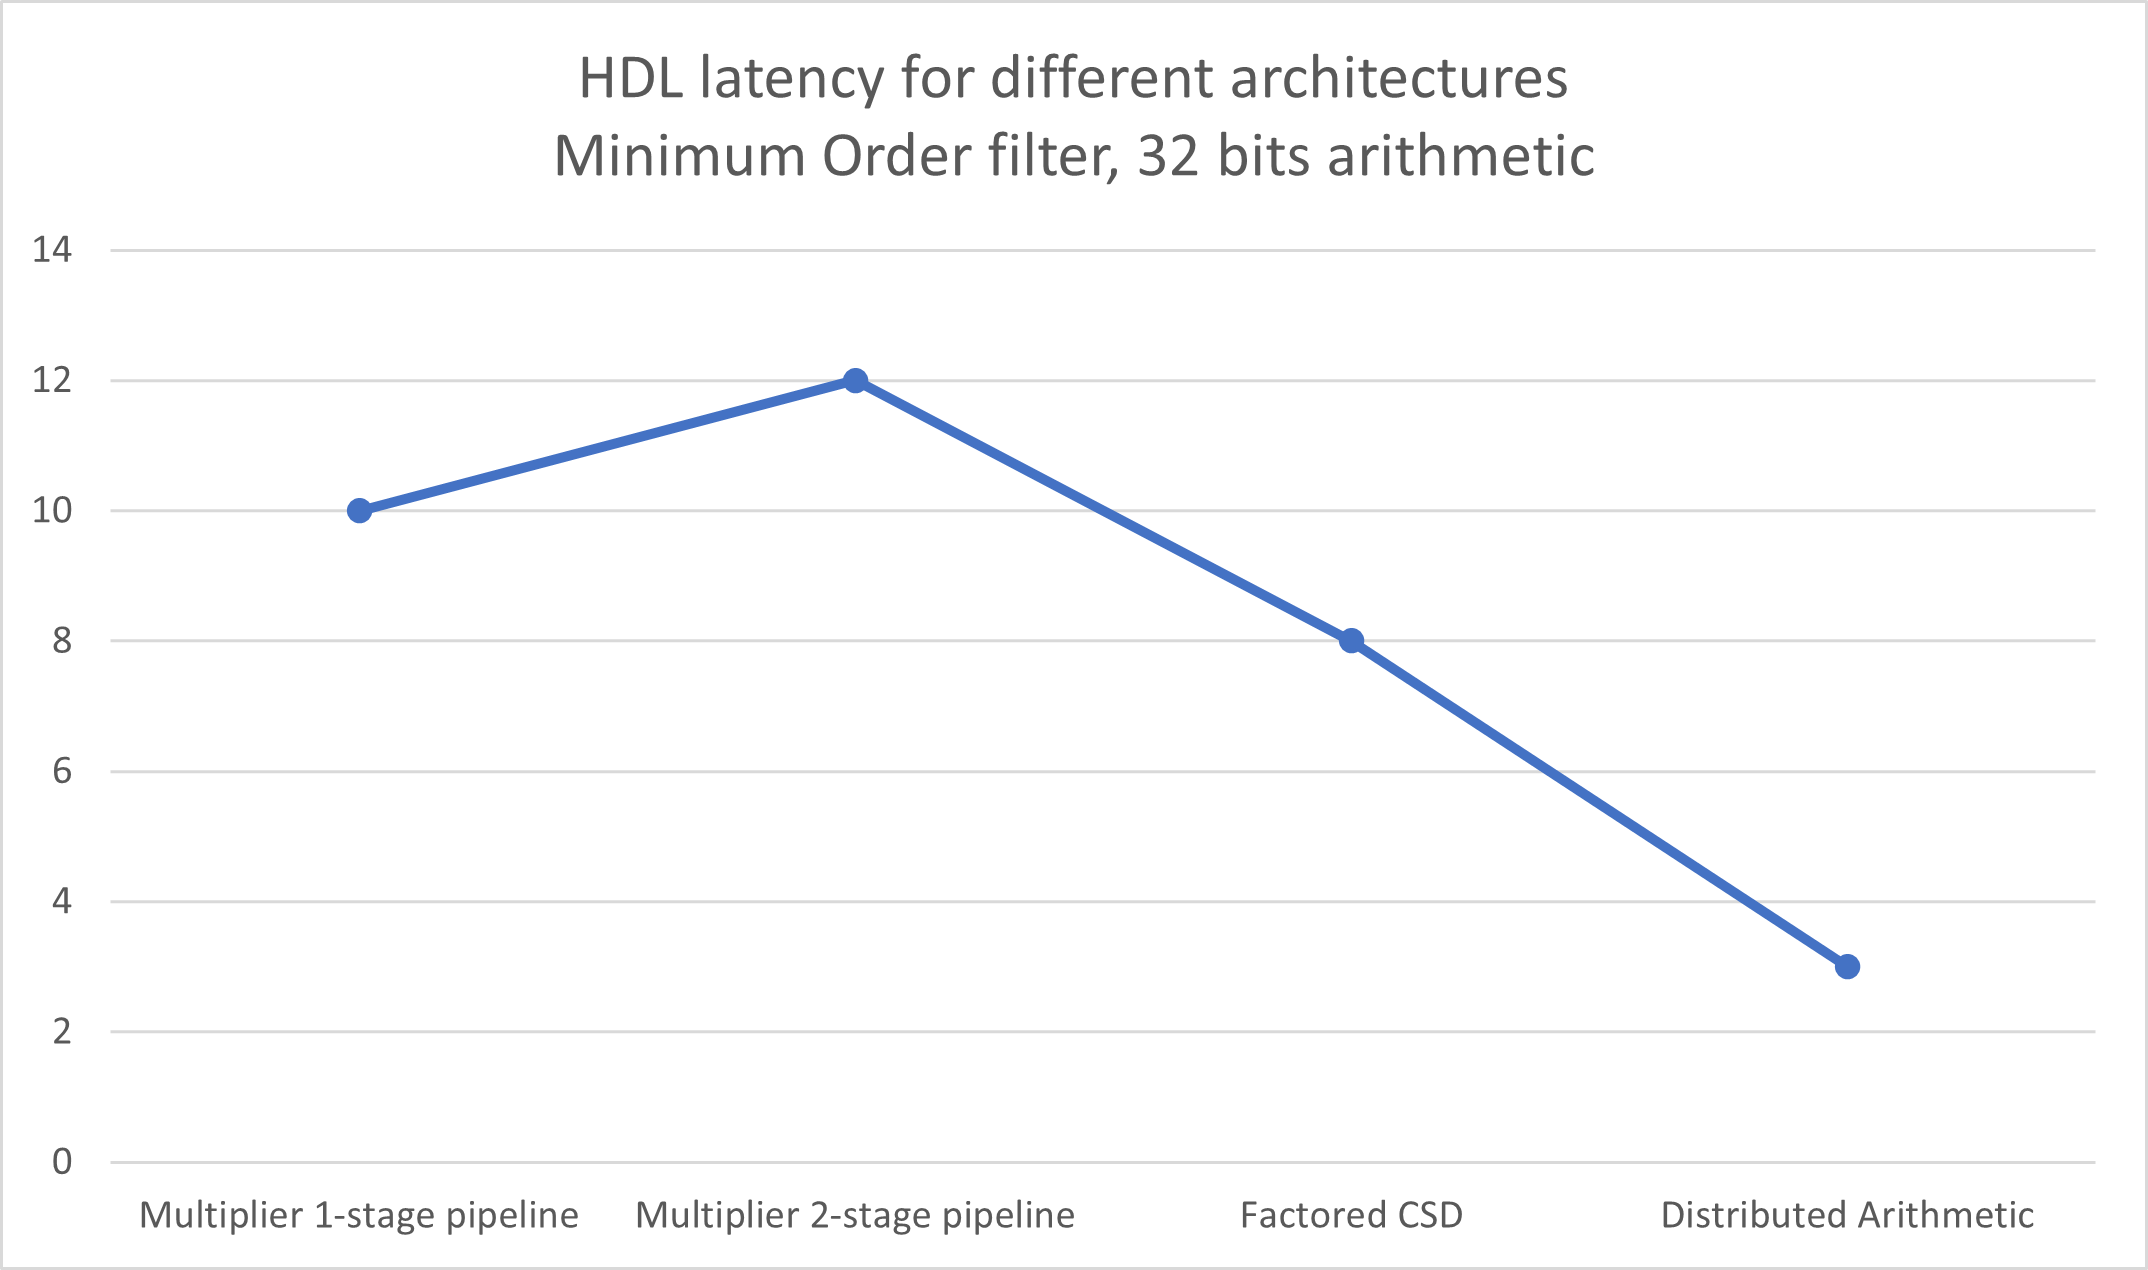
\includegraphics[width=0.45\textwidth]{../Images/FIR_min_Order/hdl_latency_32bits.png}}\\
%	\subfigure[Execution time for different architectures in seconds.]{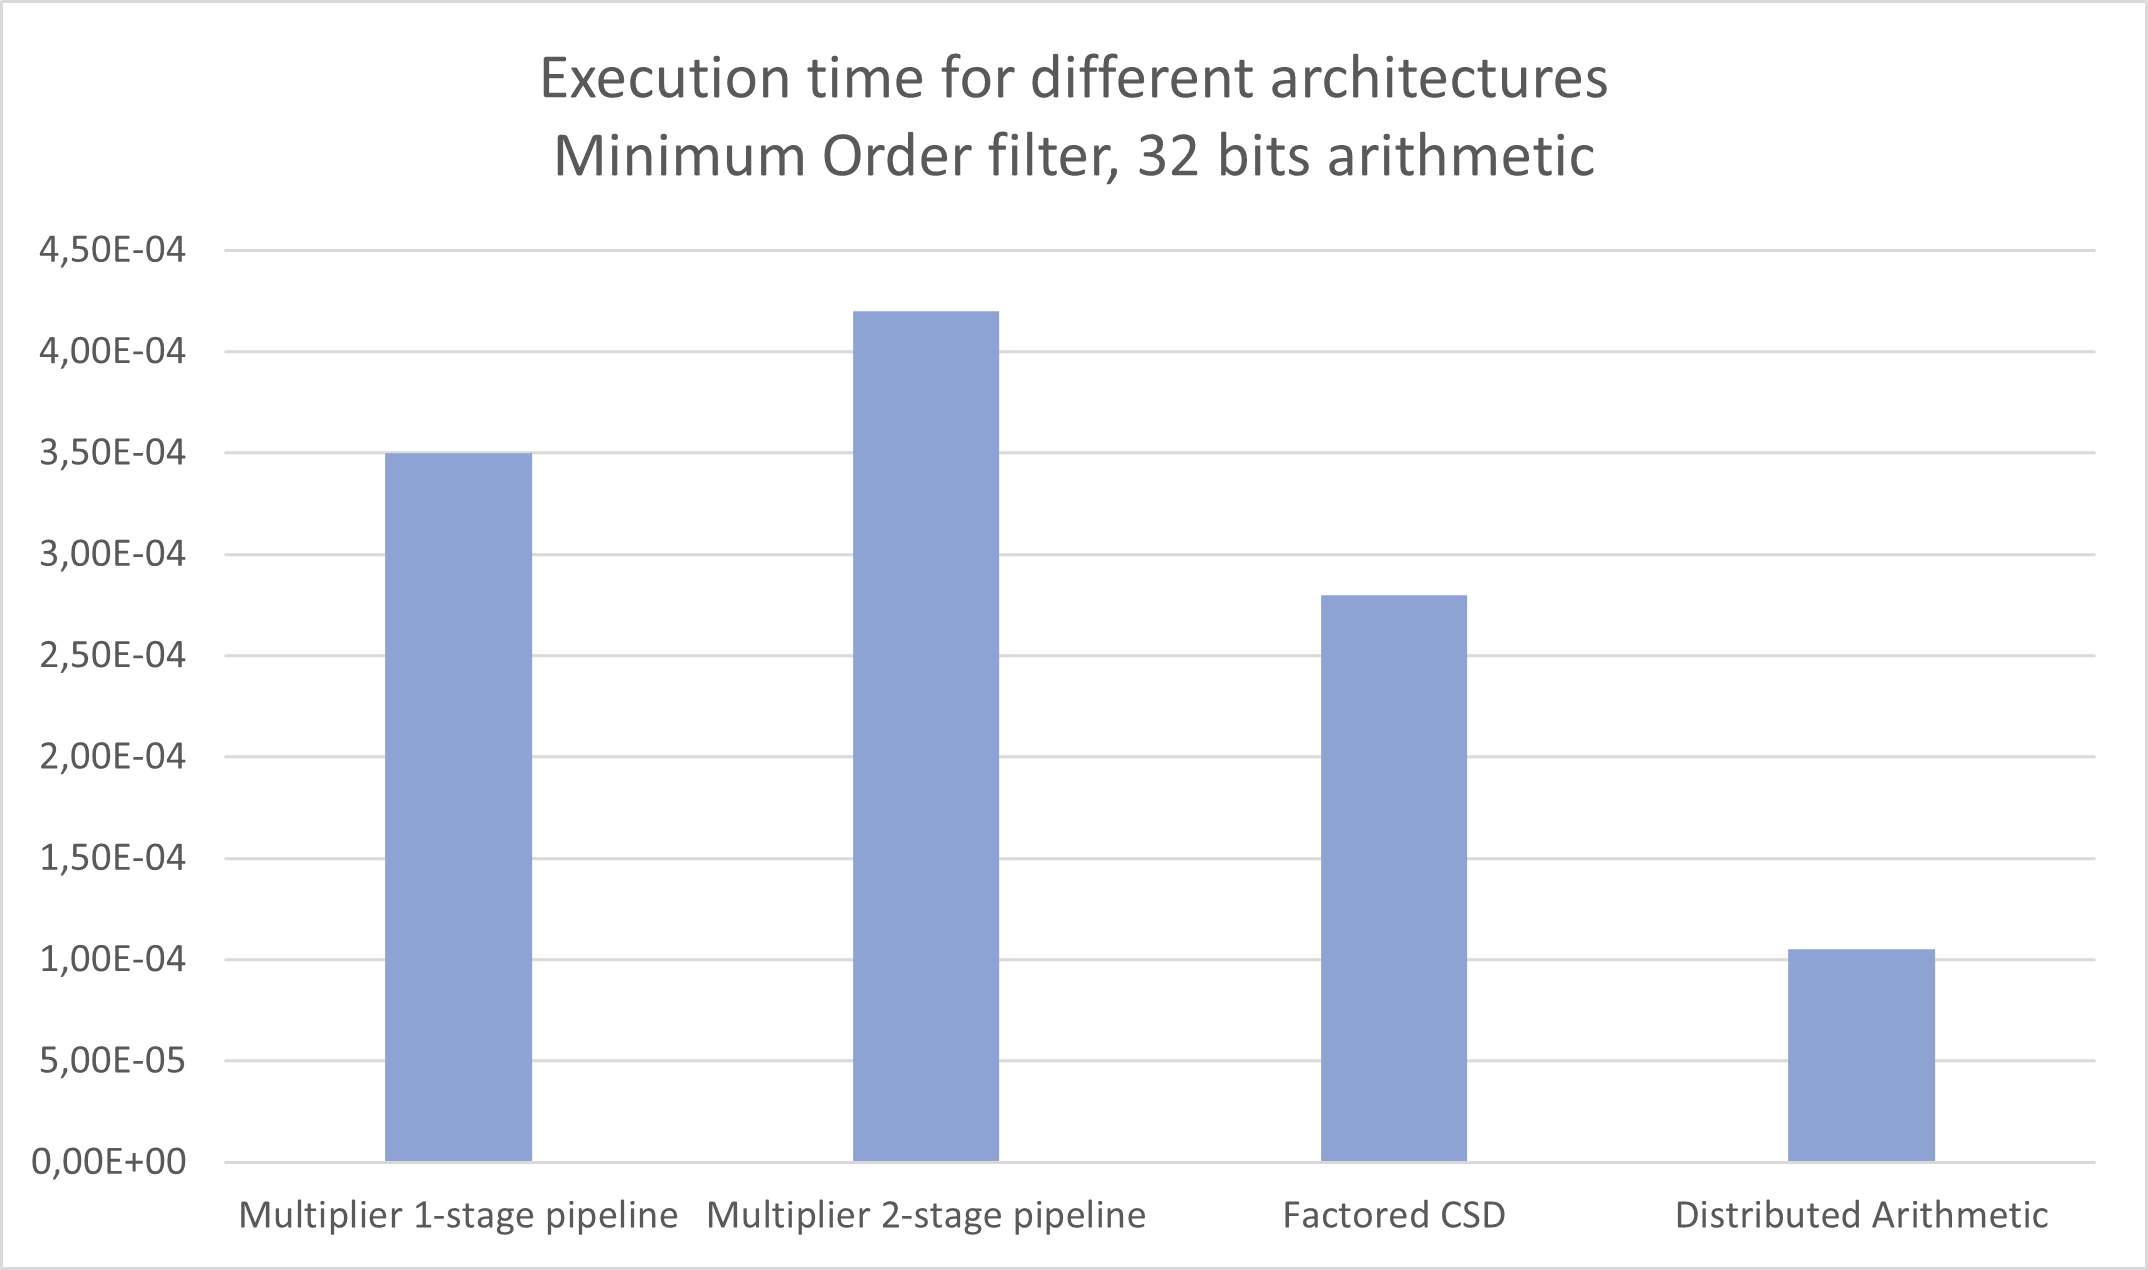
\includegraphics[width=0.45\textwidth]{../Images/FIR_min_Order/exec_time_32bits.png}}
%	\caption{Latency and execution time for different architectures.\\ \textit{Note: This is for 32bit arithmetic, the same pattern is observed for the other arithmetics.}}
%	\label{fig:exec_time_latency_min_32}
%\end{figure}

\begin{figure}[htbp]
	\centering
	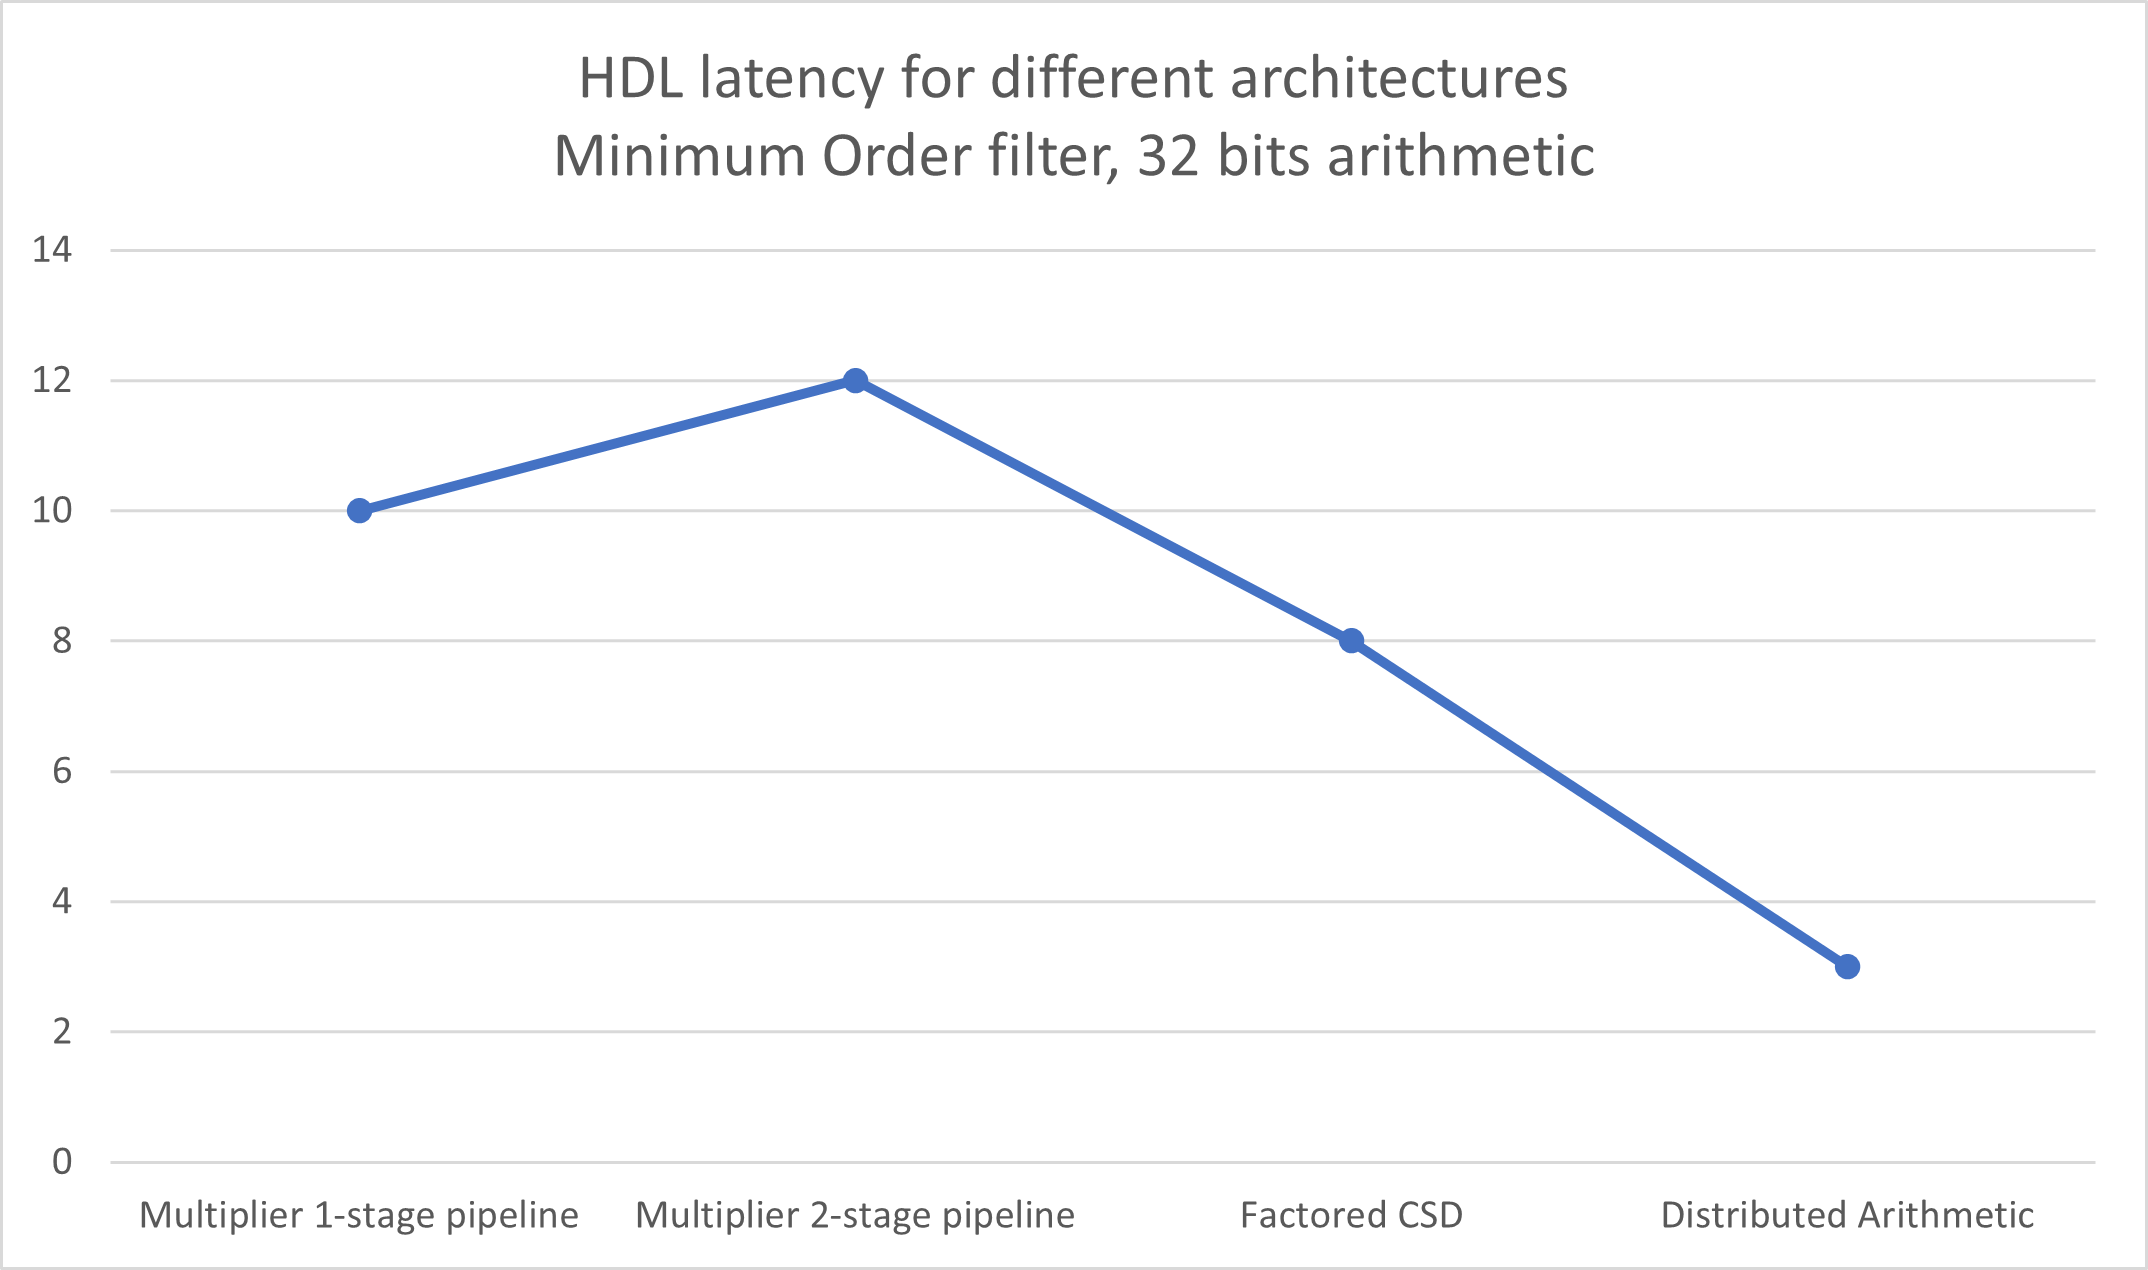
\includegraphics[width=0.45\textwidth]{../Images/FIR_min_Order/hdl_latency_32bits.png}
	\caption{HDL latency for different architectures in samples.\\ \textit{Note: This is for 32bit arithmetic, the same pattern is observed for the other arithmetics.}}
	\label{fig:hdl_latency_min_32b}
\end{figure}

\begin{figure}[htbp]
	\centering
	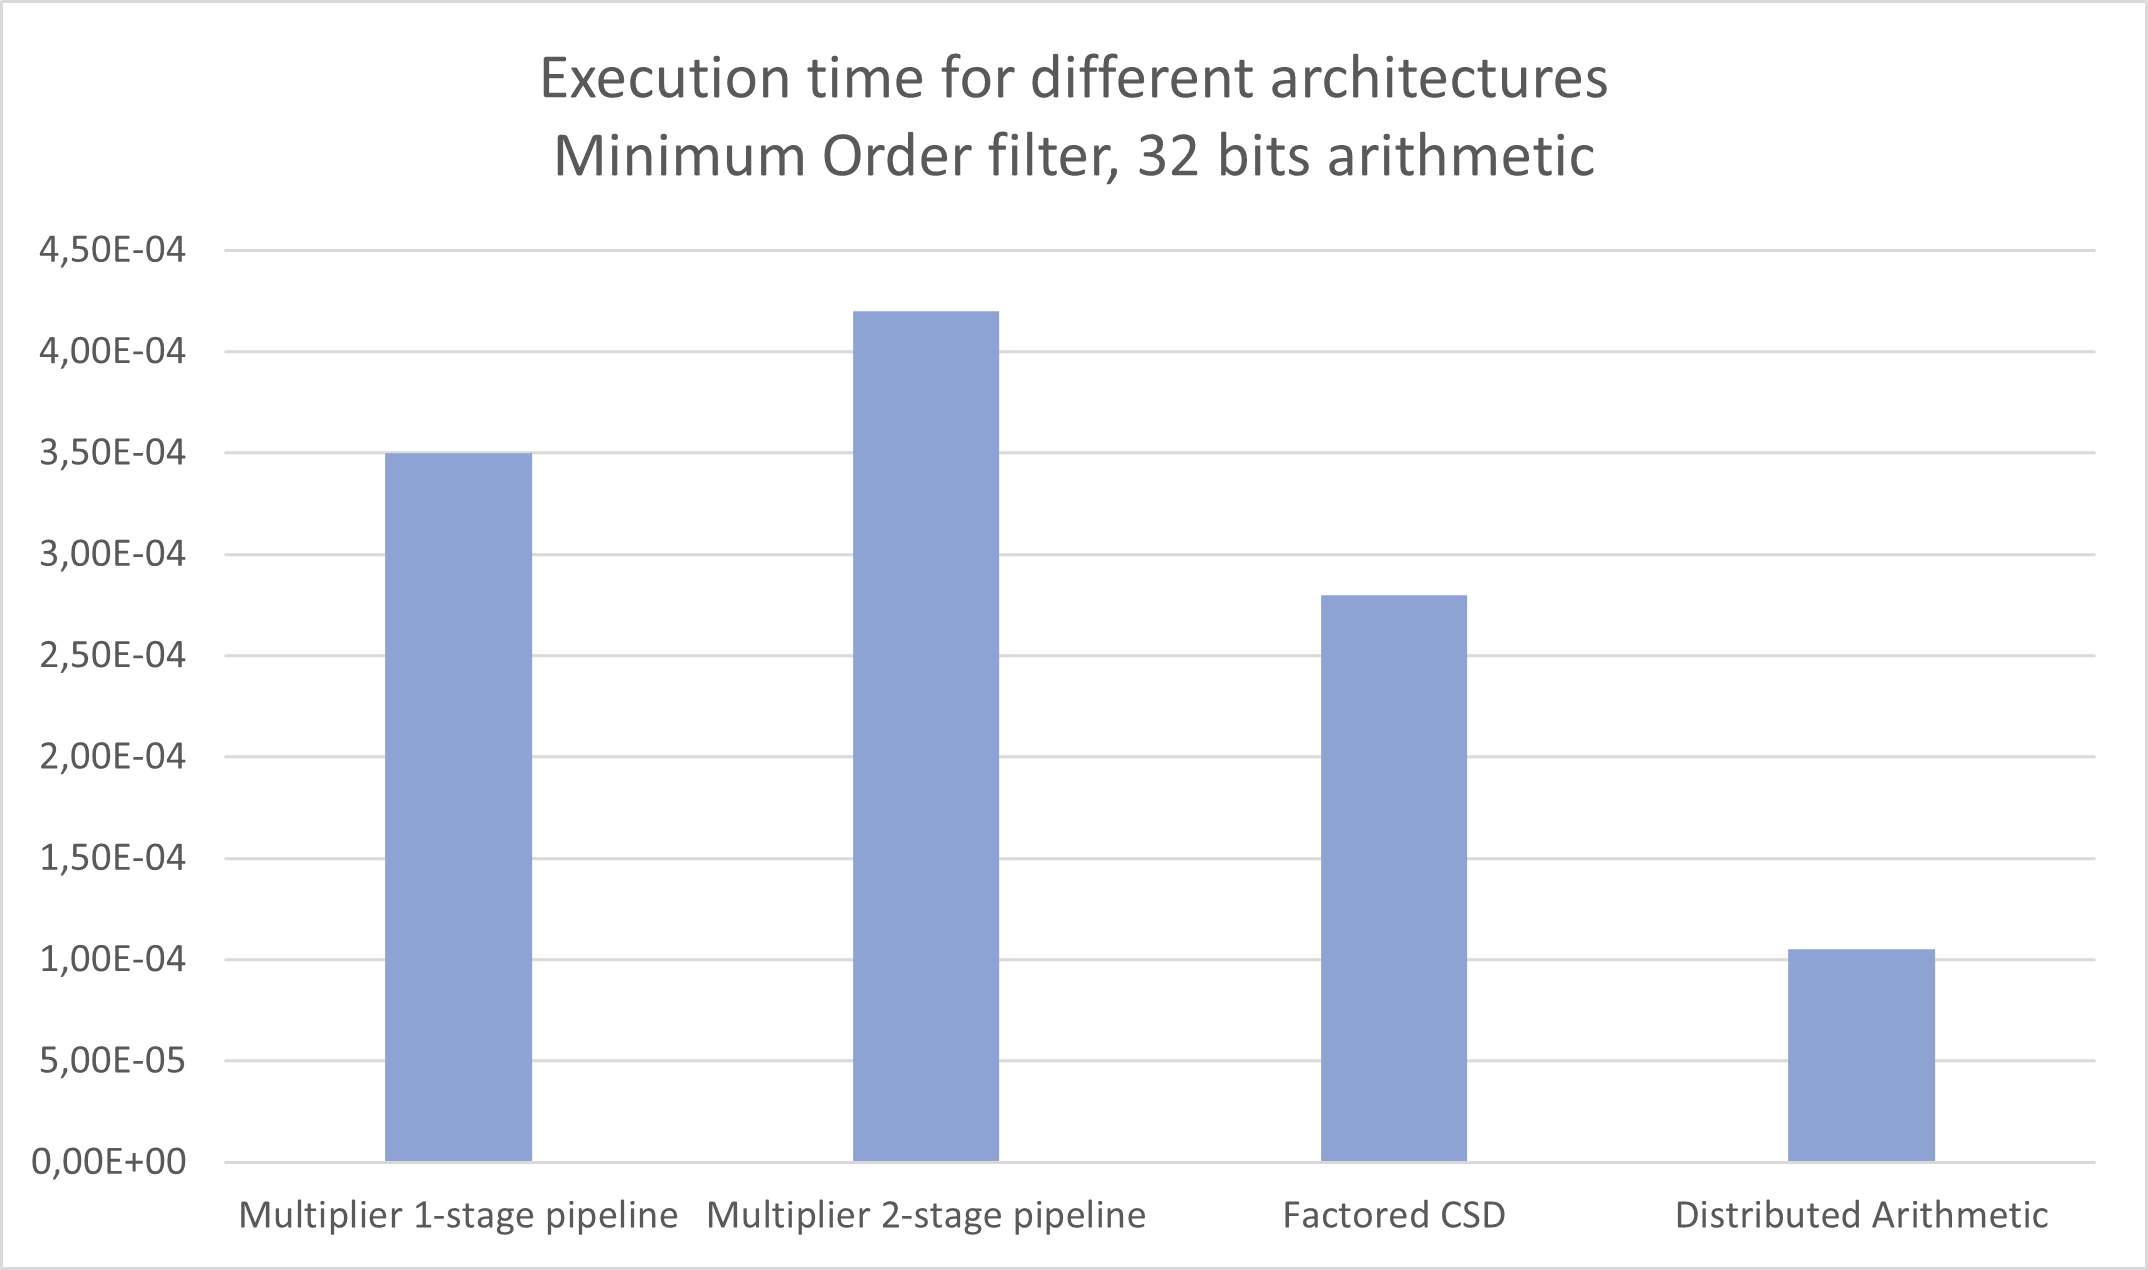
\includegraphics[width=0.45\textwidth]{../Images/FIR_min_Order/exec_time_32bits.png}
	\caption{Execution time for different architectures in seconds.}
	\label{fig:exec_time_min_32b}
\end{figure}

One of the many things changing with the reduction of the computation bit width as well as with the different arithmetic is the \verb|SNR| (\textit{Signal-to-Noise Ratio}) of the filter.
In order to measure the \verb|SNR| of the exported HDL filters, we have to run the simulation in Vivado and capture two outputs, the expected one and the actual one and import them into MATLAB for further analysis.
Then, filter expected error is calculated by subtracting the expected output from the actual one and by calling the \verb|snr()| function we get the Signal to Noise Ratio to compare different arithmetics and architectures.

Figure~\ref{fig:fir_min_snr} shows SNR values for this filter across multiple arithmetic bit-width and architectures. We can observe that SNR relatively stays the same for both multiplier architectures and multiplier-less CSD with values around $30.2 \hspace{3pt} dB$, with only DA having a very small value of $6.5 \hspace{3pt} dB$.
This trend is followed for every bit width and is caused by the "bad" filter capabilities of the generated filter. Seeing the magnitude response of it in fig~\ref{fig:min_order_filt}, we can clearly see that even from $0$ Hz, magnitude is already at $-50 \hspace{3pt} dB$ which is not desired. If we were to add the losses of some architectures, as described in section~\ref{sec:filter_comp_subsec:architectural_diff}, those numbers start to appear normal.

\begin{figure}[htbp]
	\centering
	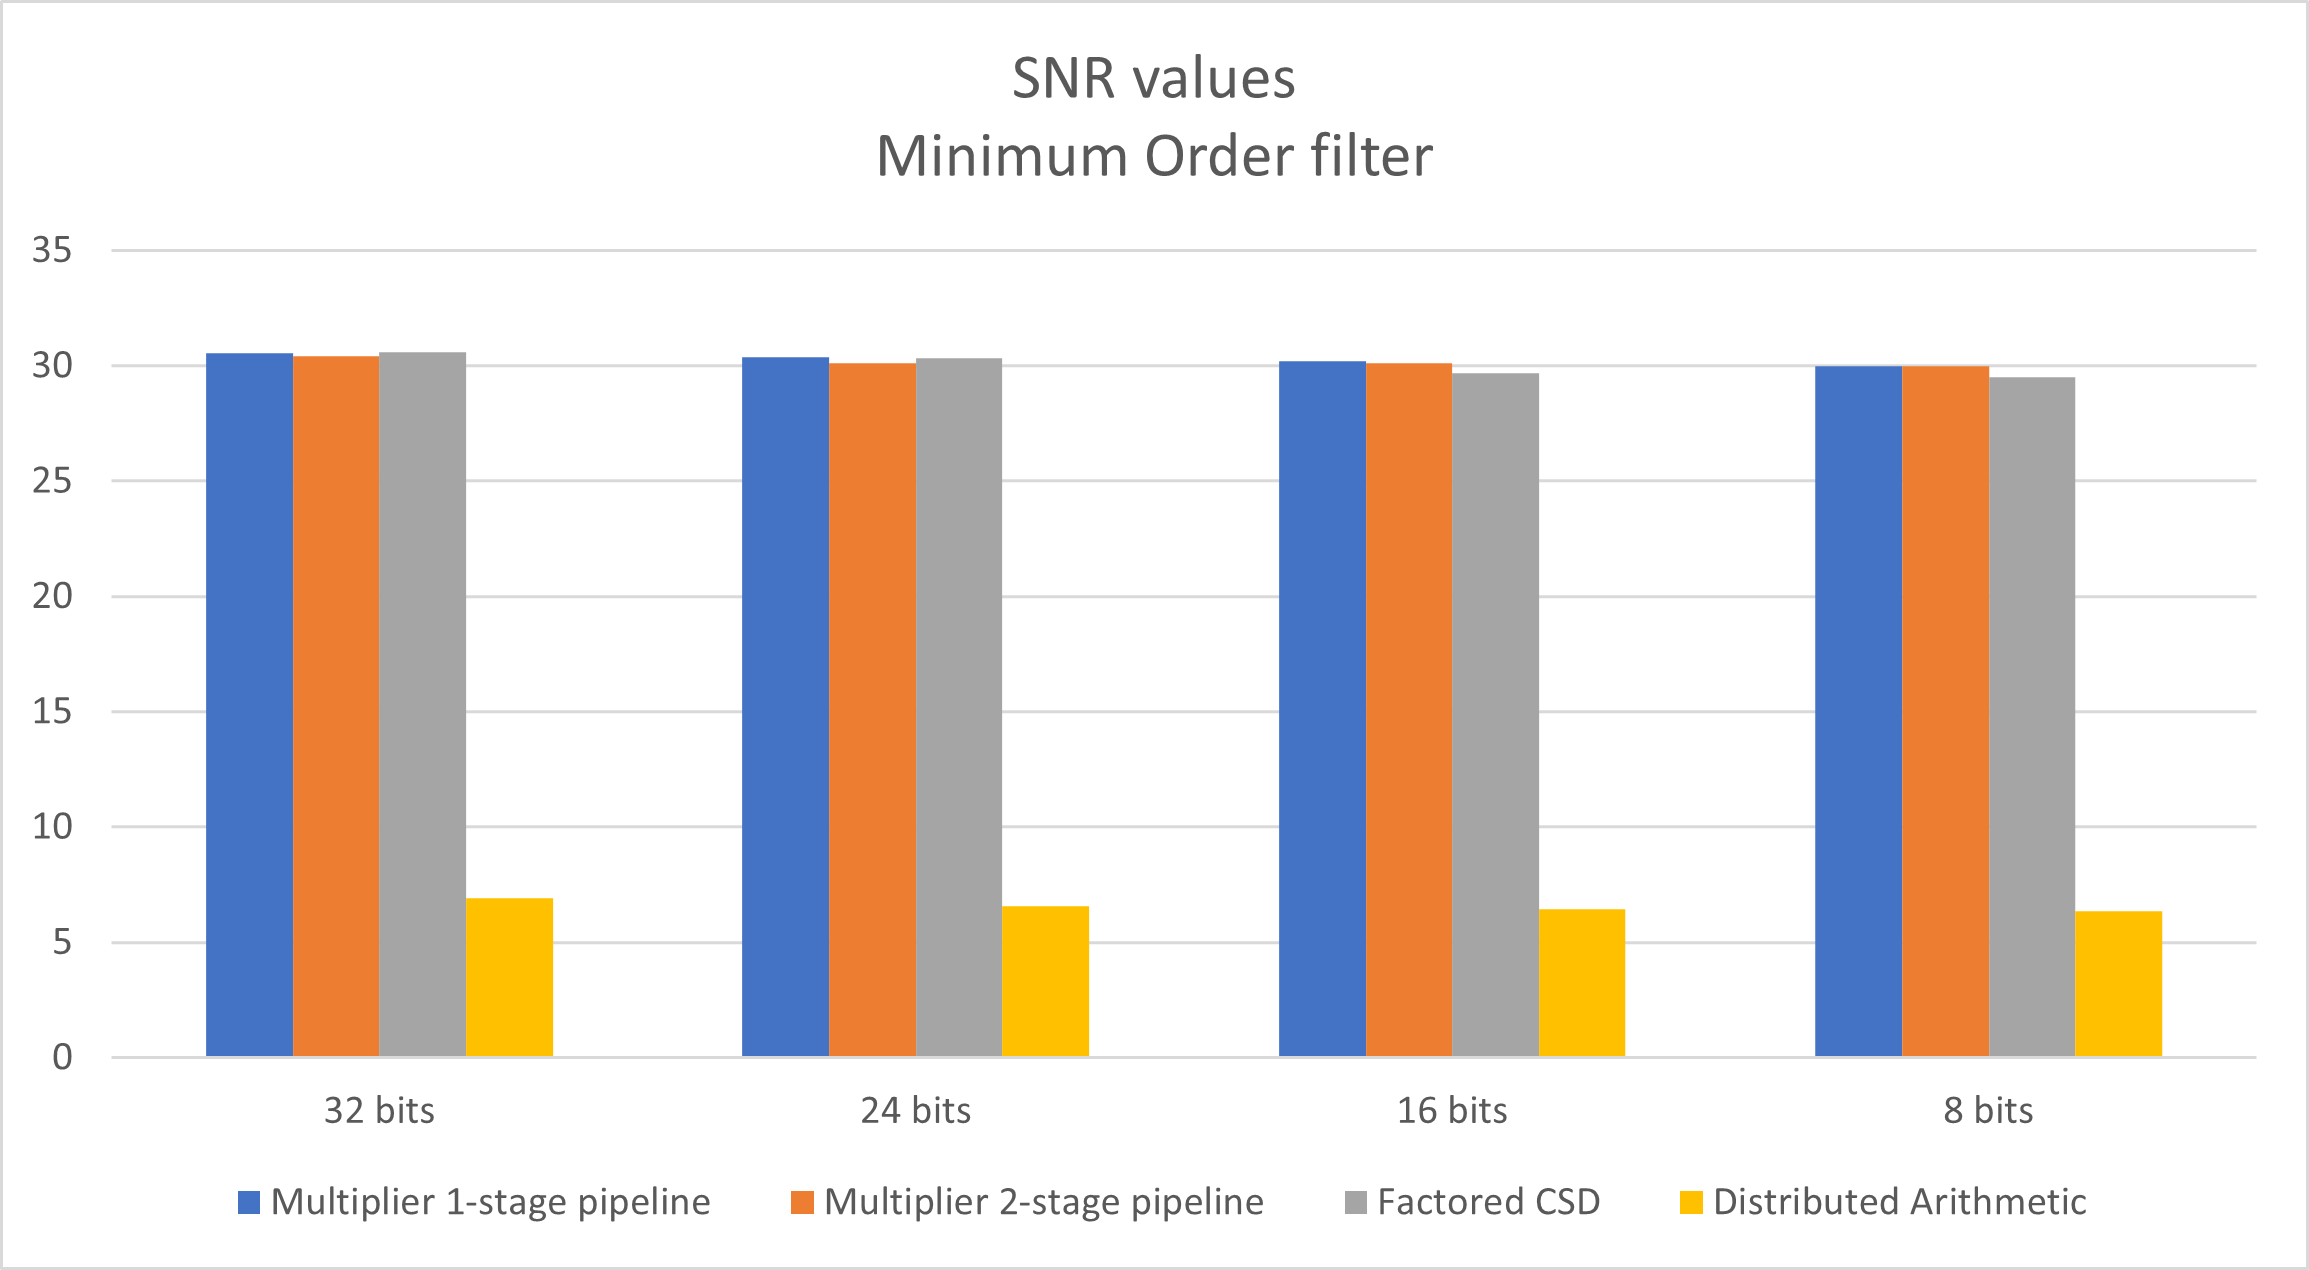
\includegraphics[width=0.45\textwidth]{../Images/FIR_min_Order/snr_values.png}
	\caption{SNR values of the minimum coefficient filter}
	\label{fig:fir_min_snr}
\end{figure}

Finally, while the distributed arithmetic architecture seems to be the most quick of all above architectures as viewed in figure~\ref{fig:exec_time_min_32b} for a specific arithmetic bit width and appears to be the most efficient of all (since LUT and flip flop utilizations are smaller than that of other architectures), it clearly isn't the correct one. This is the cost of every approximation technique applied by the architecture.
Those approximations introduce errors that are more significant from those introduced in factored CSD architecture since those errors accumulate throughout the computation stages. Each stage involves a lookup operation and subsequent accumulation of values thus its impact is bigger on overall system accuracy.

\subsection{20$^{th}$ Order filter}
Moving to a filter which uses more coefficients, filtering capabilities are becoming much better.

Starting with execution times in figure~\ref{fig:fir_20_hdl_latency}, we can clearly see the same pattern occurred in the previous filter. Both sample latency and execution times have almost the same gradients and this is normal, as the only thing changing is the operations per sample (\textit{increased to 41 from 7 in min. \hspace{-10pt} order filter}). As we change architectures from multiplier to multiplier-less (\textit{either f-CSD or DA}), the number of operations per sample increase but multiplication is not taking place. These operations are generally additions which are more cheap to implement (\textit{mainly implemented using LUTs}).

Utilization also increased, since more computations are executed in one sample cycle.
The filter order directly corresponds to the number of filter taps or coefficients used in the design. As the filter order increases, more taps are required to achieve the desired frequency response and filtering characteristics.

\begin{figure}[htpb]
	\centering
	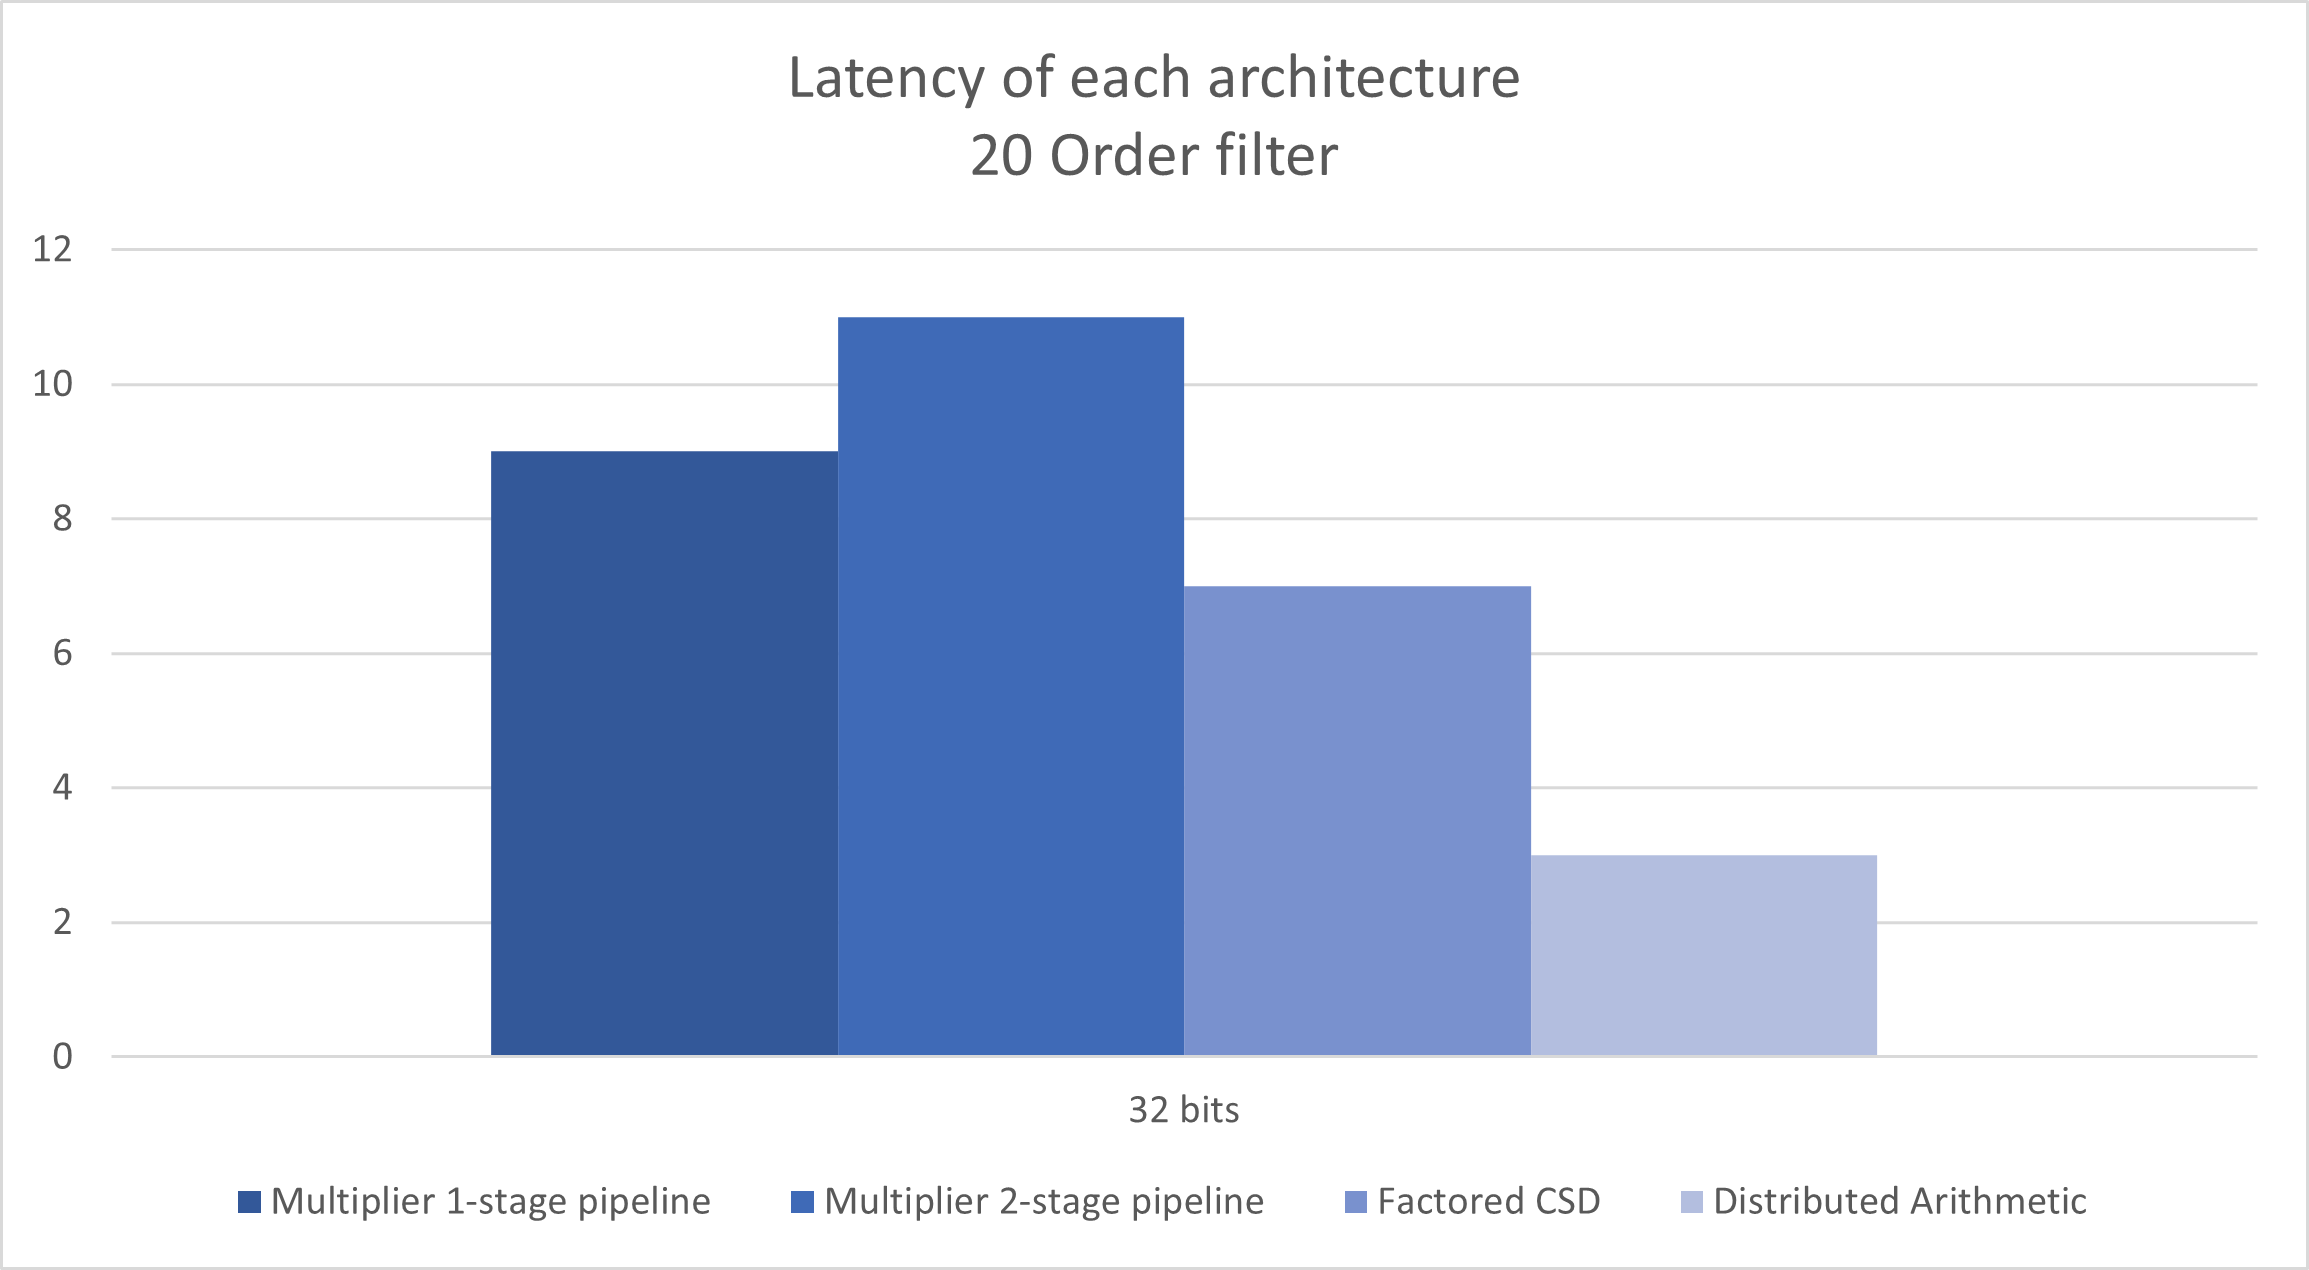
\includegraphics[width=0.45\textwidth]{../Images/FIR_20_Order/hdl_latency.png}
	\caption{Latency per sample for different architectures.}
	\label{fig:fir_20_hdl_latency}
\end{figure}

As far as SNR values are concerned, there is an improvement over the previous filter in both consistency and magnitude of numbers. Beginning with multiplier architectures, we observe a solid $\approx 38 \hspace{3pt} dB$ value for both 32 and 24 bits with steadily decreasing values for 16 and 8 bits arithmetic width ($\approx 34 \hspace{3pt} dB$).

\begin{figure}
	\centering
	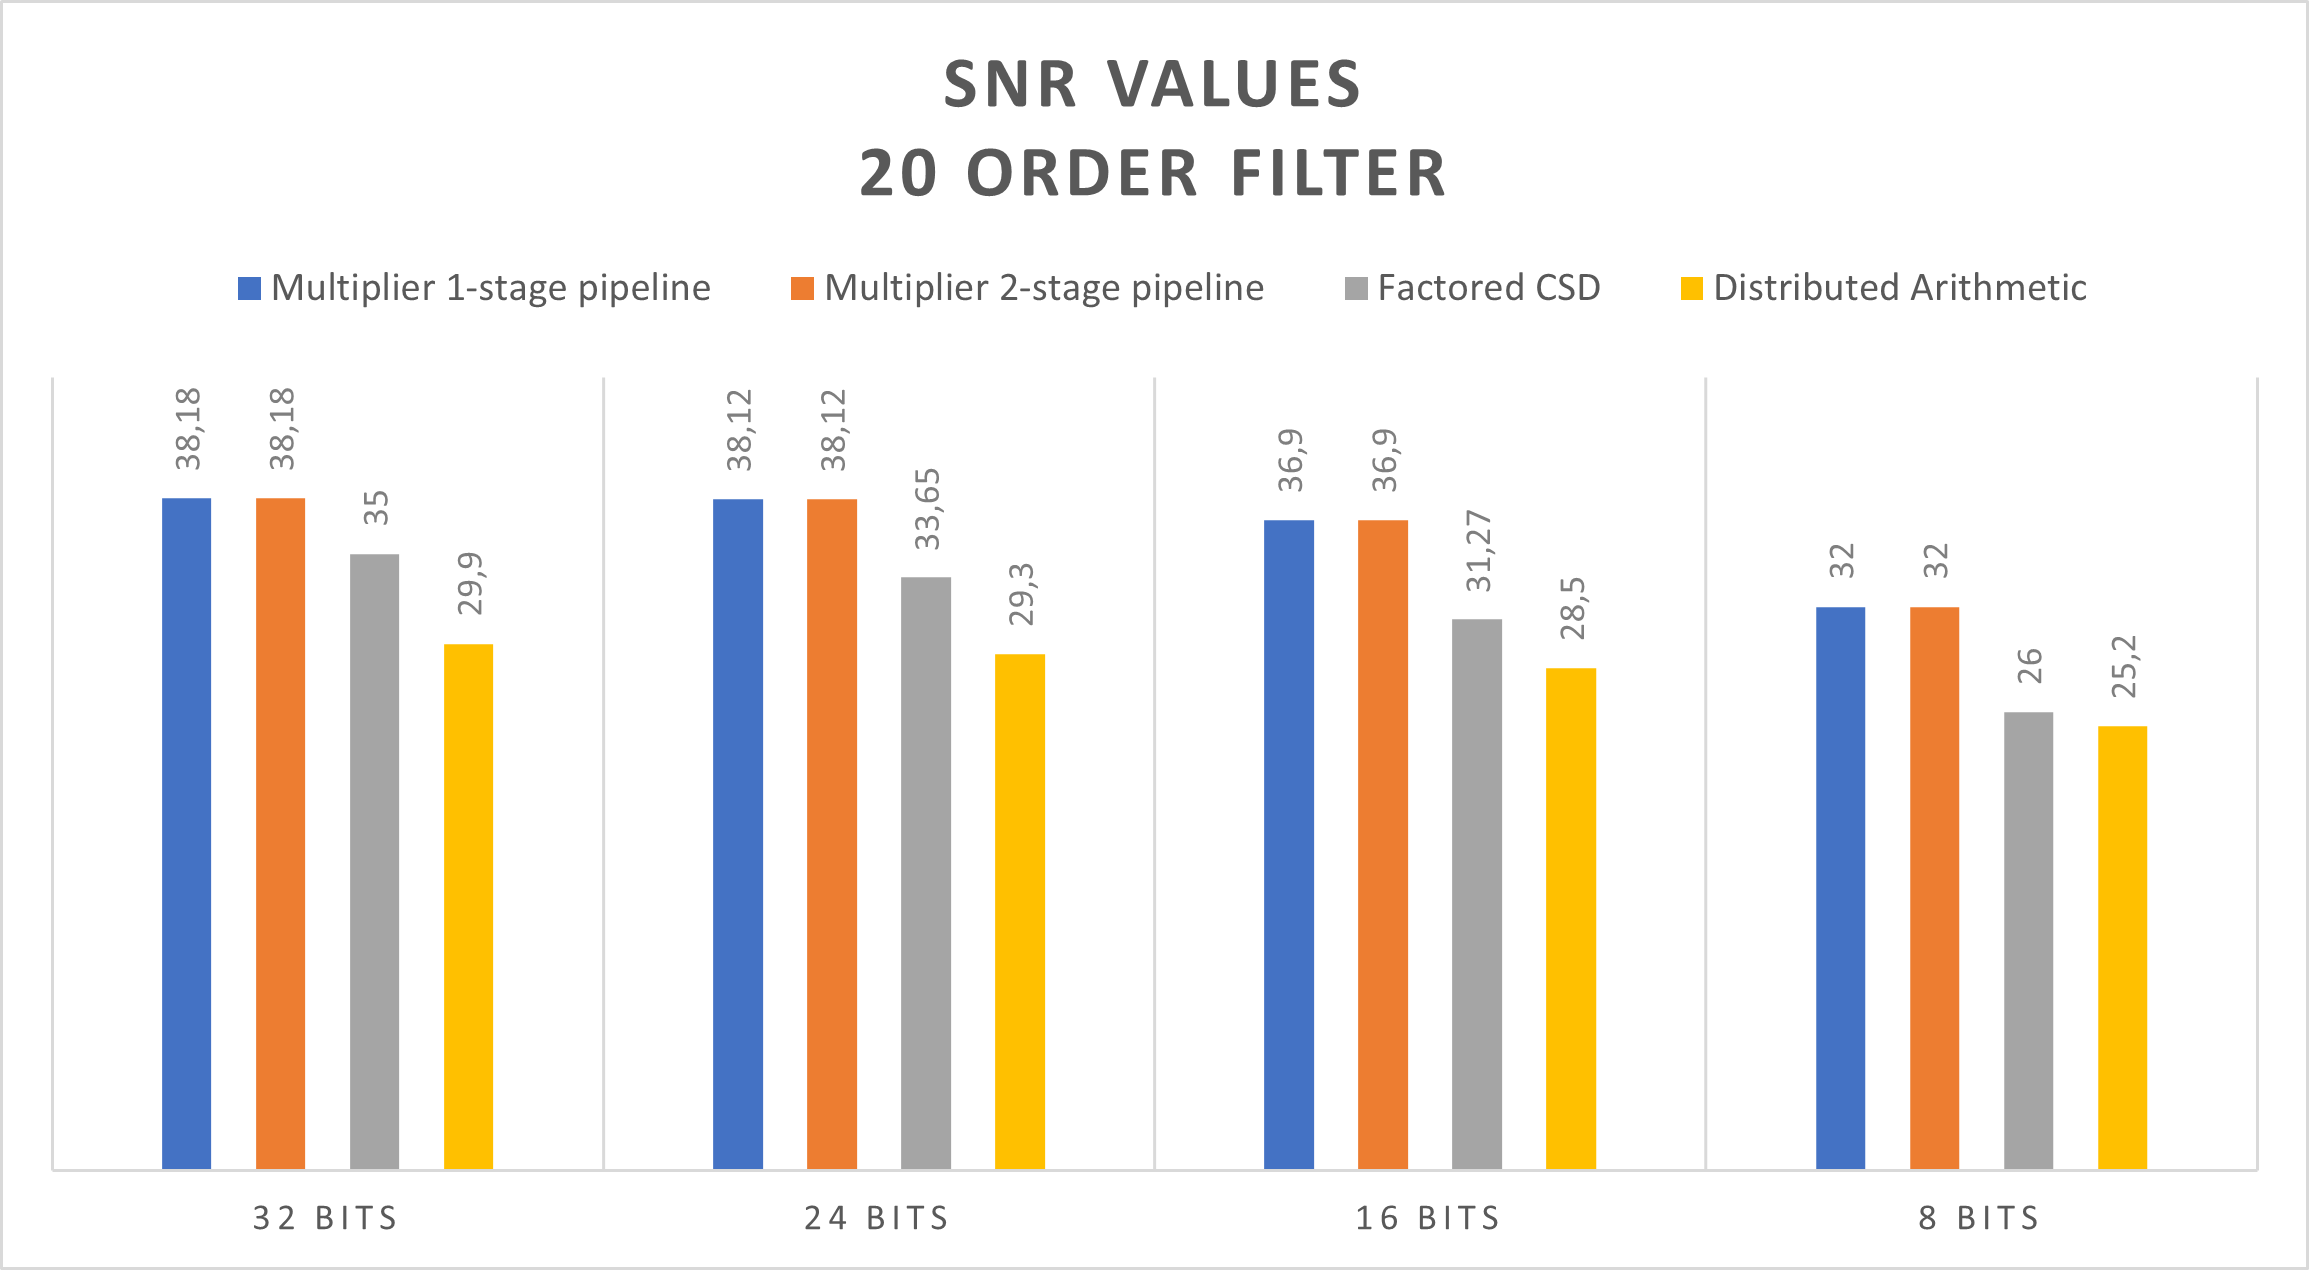
\includegraphics[width=0.45\textwidth]{../Images/FIR_20_Order/snr_values.png}
	\caption{SNR values of 20 order filter for different arithmetics.}
	\label{fig:fir_20_snr}
\end{figure}

\subsection{30$^{th}$ Order filter}
The 30$^{th}$ order filter is itself a better representation of the 20$^{th}$ order one.
Once again, increasing the order of a filter raises the number of operations due to the increased complexity of the filter structure.
The order of a filter refers to the number of filter taps or coefficients used in the design, which directly affects the number of mathematical operations required to process the input signal, thus increasing the overall utilization further across every architecture.

Being a higher order, the filter has a narrower transition band and steeper roll-off characteristics, enabling it to suppress unwanted noise more effectively. This can result in an improved SNR, as the filter can better separate the desired signal from the noise. The above theory can indeed be observed in figure~\ref{fig:fir_30_snr}.

SNR magnitude for multiplier architectures lies around $\approx 42 \hspace{3pt} dB$ while it is reduced for the non-multiplier (\emph{approximation}) architectures. For relatively large bit-width (\emph{32, 24 bits}), all architectures have almost the same SNR value except dsitributed arithmetic's value which is $\approx8 \hspace{3pt} dB$ smaller everywhere. While transitioning to the lowest bit width arithmetics (\emph{16, 8 bits}), the approximation trade-offs start to appear a bit clearer.
Both factored-CSD and distributed arithmetic have significantly smaller SNR number for those bit-widths compared with multiplier ones, but at the same time they require less hardware to operate as fig.~\ref{fig:lut_ff_util_all} indicate.

As far as performance is concerned, this filter has the same latency per sample as the 20$^{th}$ one, thus having the same execution time for the same sample set. This happens because the number of operations has increased to a point where the calculations can be completed within the same time as the 20$^{th}$ order one.


\begin{figure}[htpb]
	\centering
	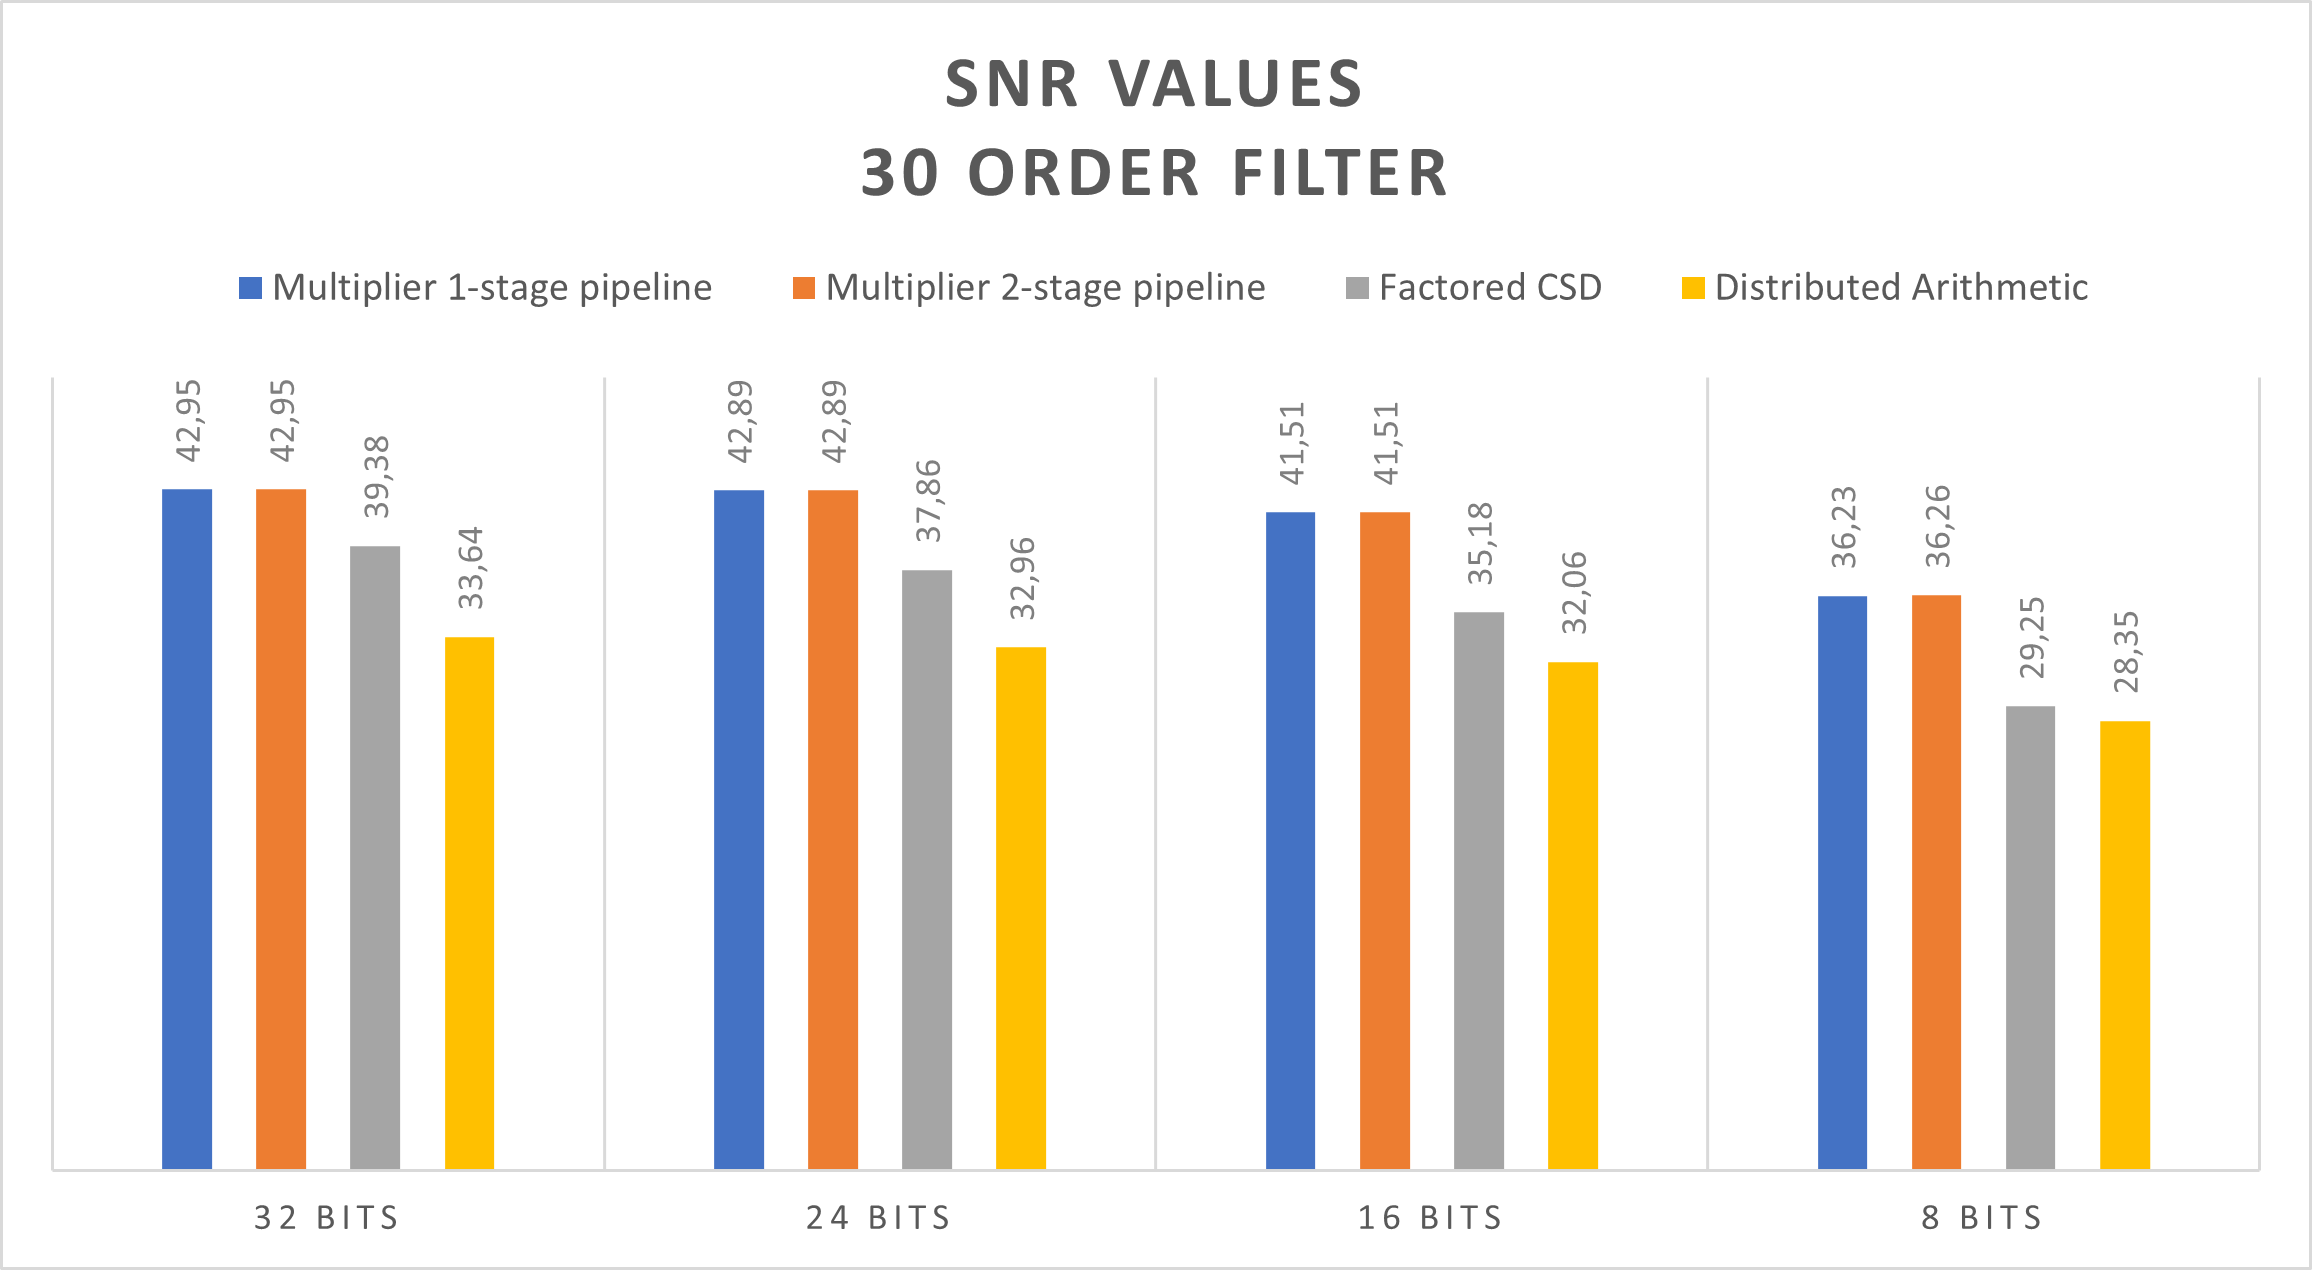
\includegraphics[width=0.45\textwidth]{../Images/FIR_30_Order/snr_values.png}
	\caption{SNR values of 30$^{th}$ order filter.}
	\label{fig:fir_30_snr}
\end{figure}

\subsection{Overall utilizations}
Overall utilizations can be observed in figure complex~\ref{fig:lut_ff_util_all}.
\begin{figure*}[h]
	\centering
	\subfigure[FF utilization of min order filter]{
		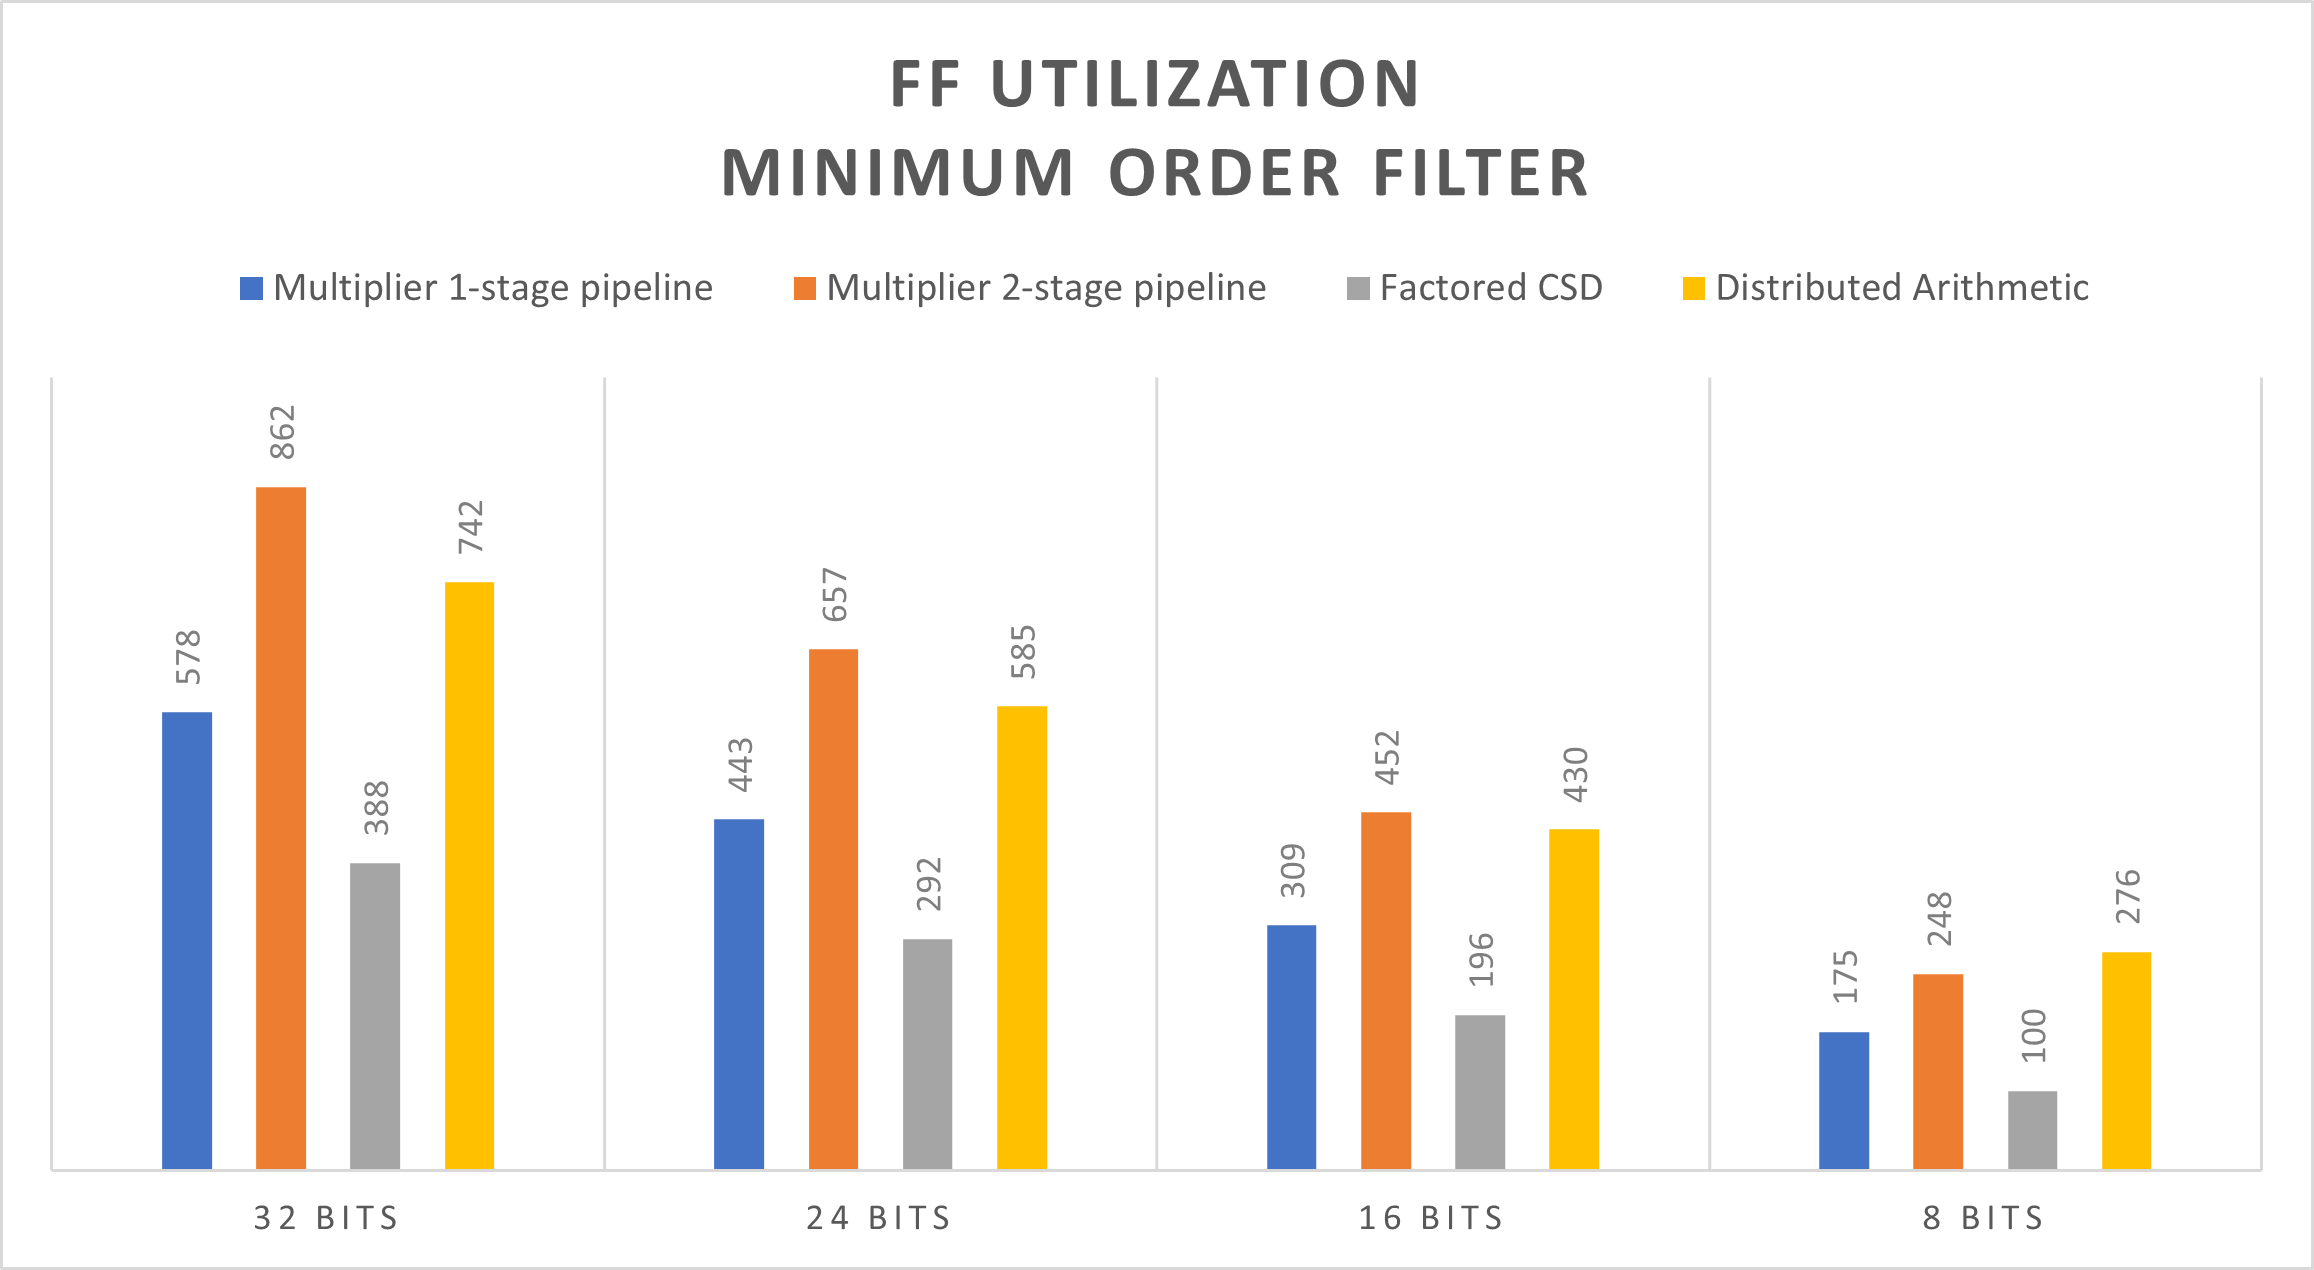
\includegraphics[width=0.45\textwidth]{../Images/FIR_min_Order/ff_utilization.png}
	}
	\subfigure[LUT utilization of min order filter]{
		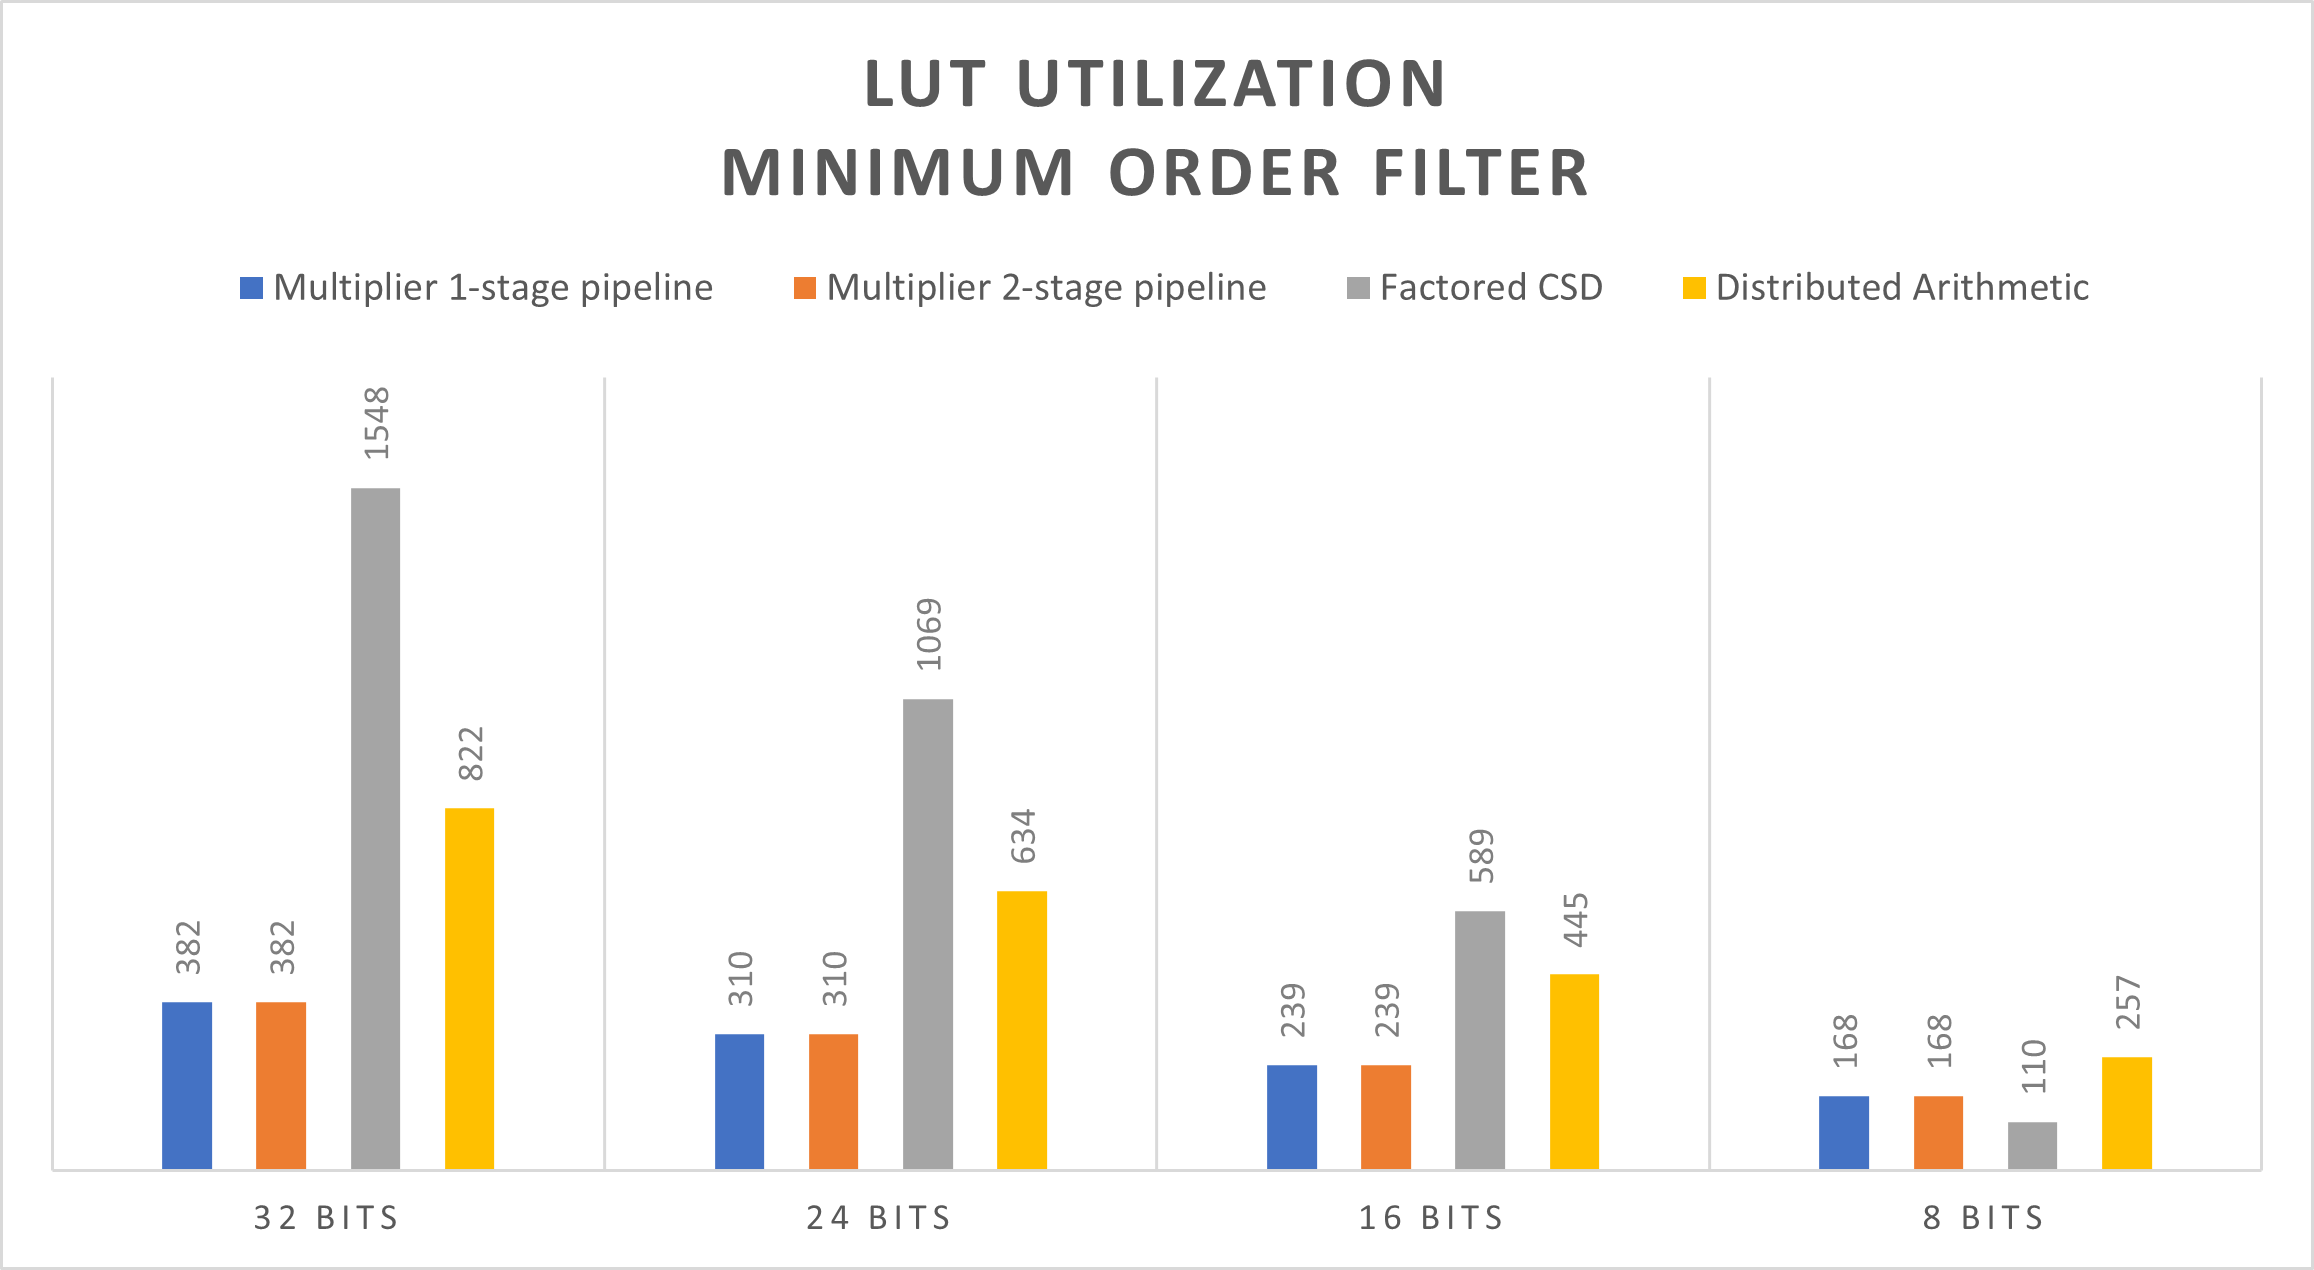
\includegraphics[width=0.45\textwidth]{../Images/FIR_min_Order/lut_utilization.png}
	}
	\subfigure[FF utilization of 20 order filter]{
		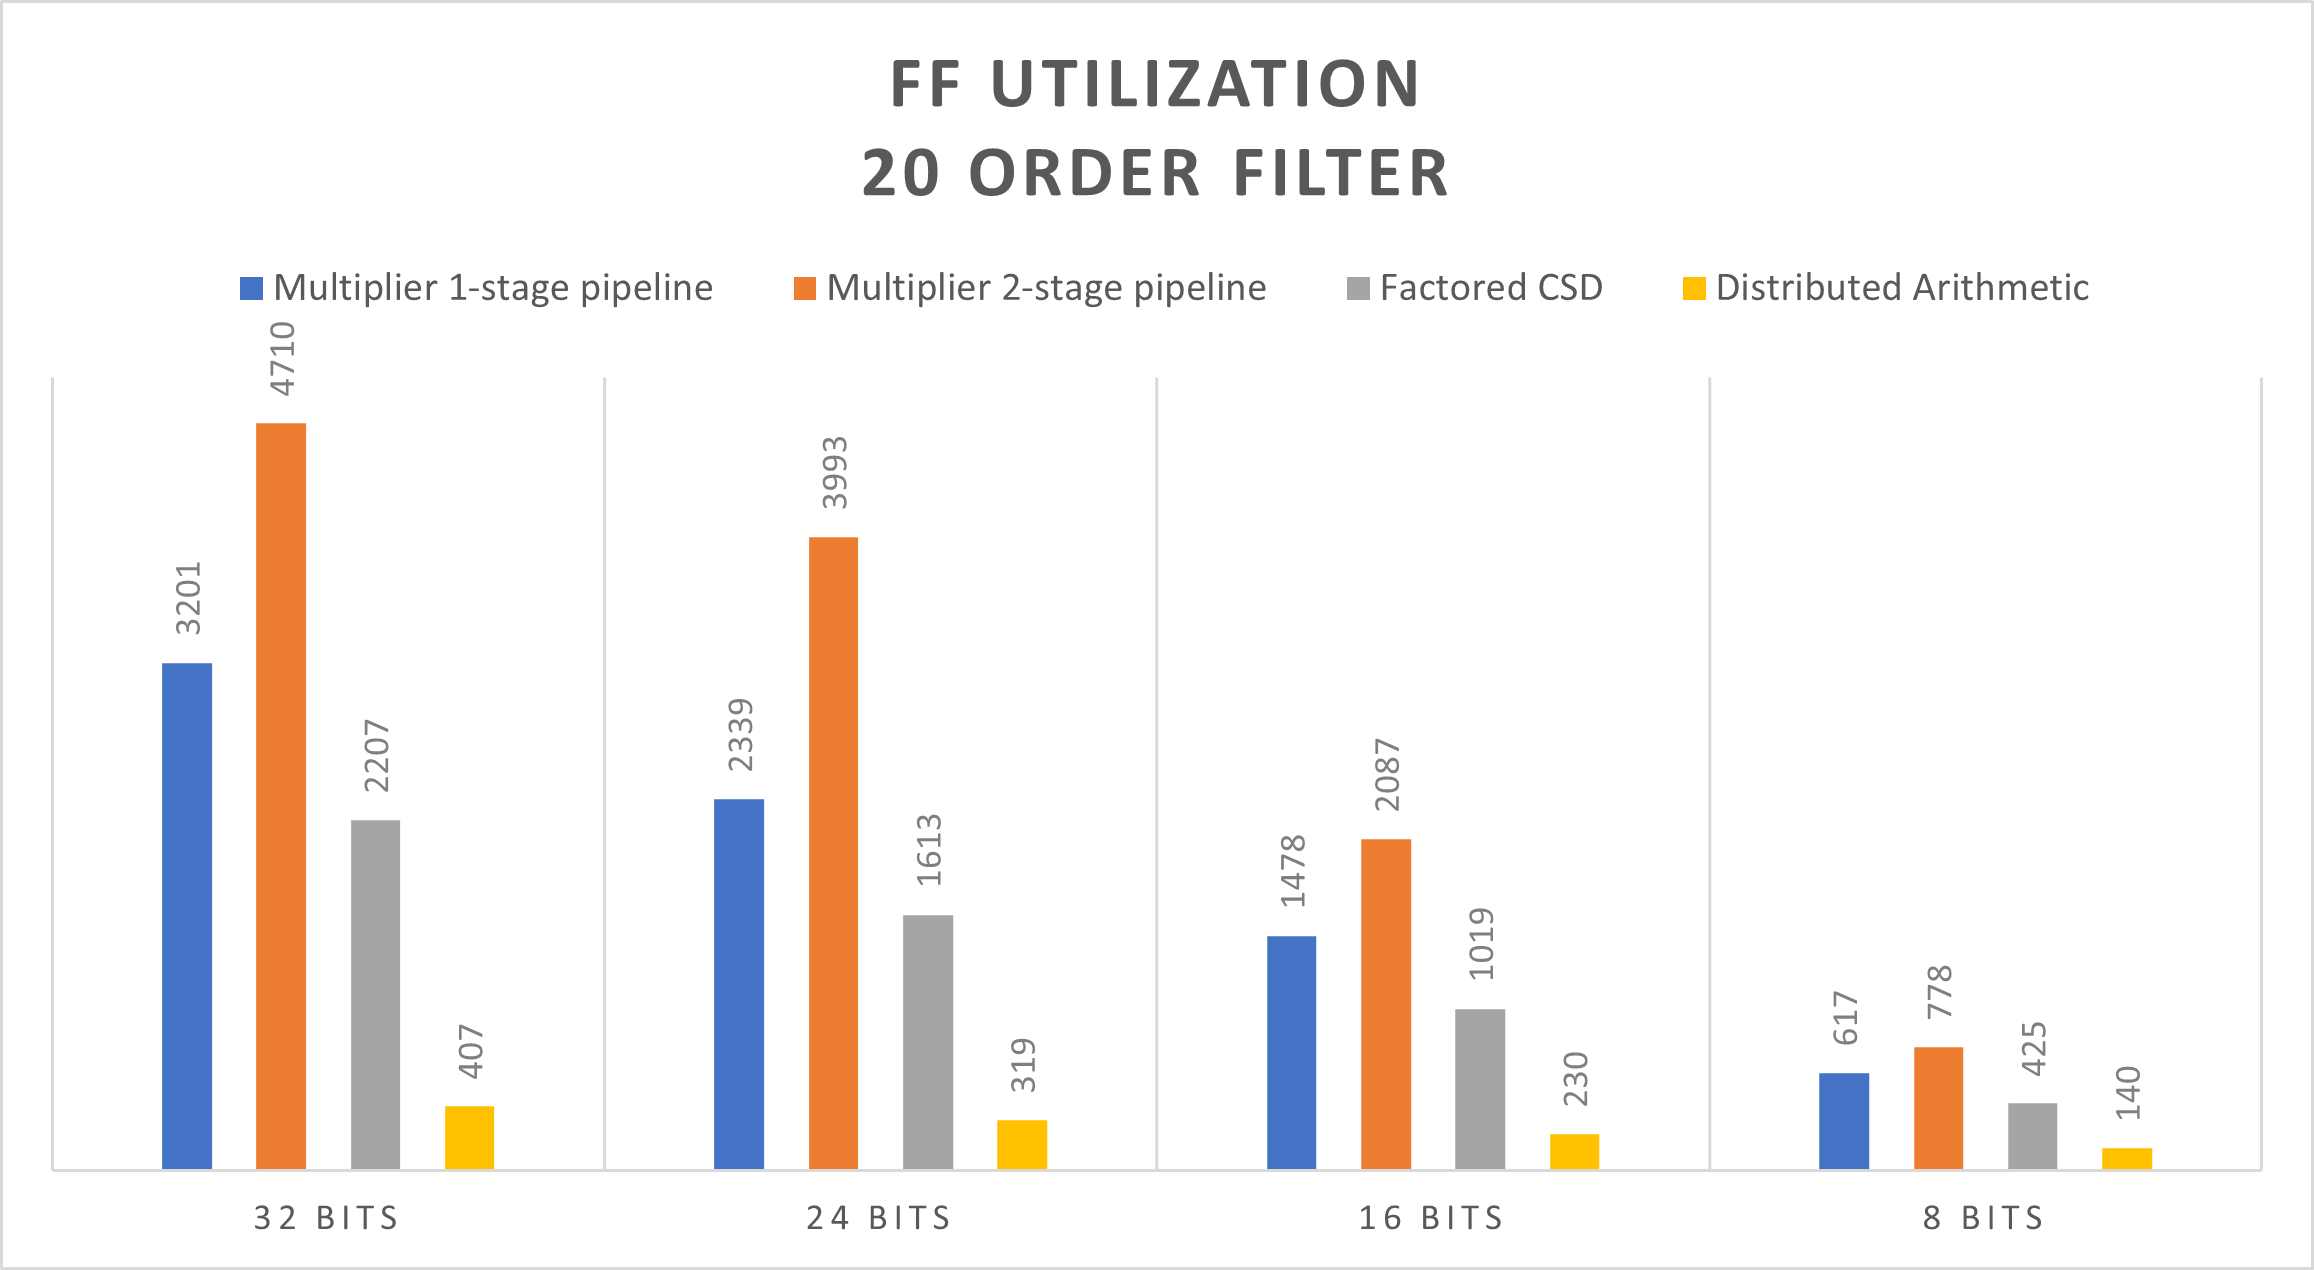
\includegraphics[width=0.45\textwidth]{../Images/FIR_20_Order/ff_utilization.png}
	}
	\subfigure[LUT utilization of 20 order filter]{
		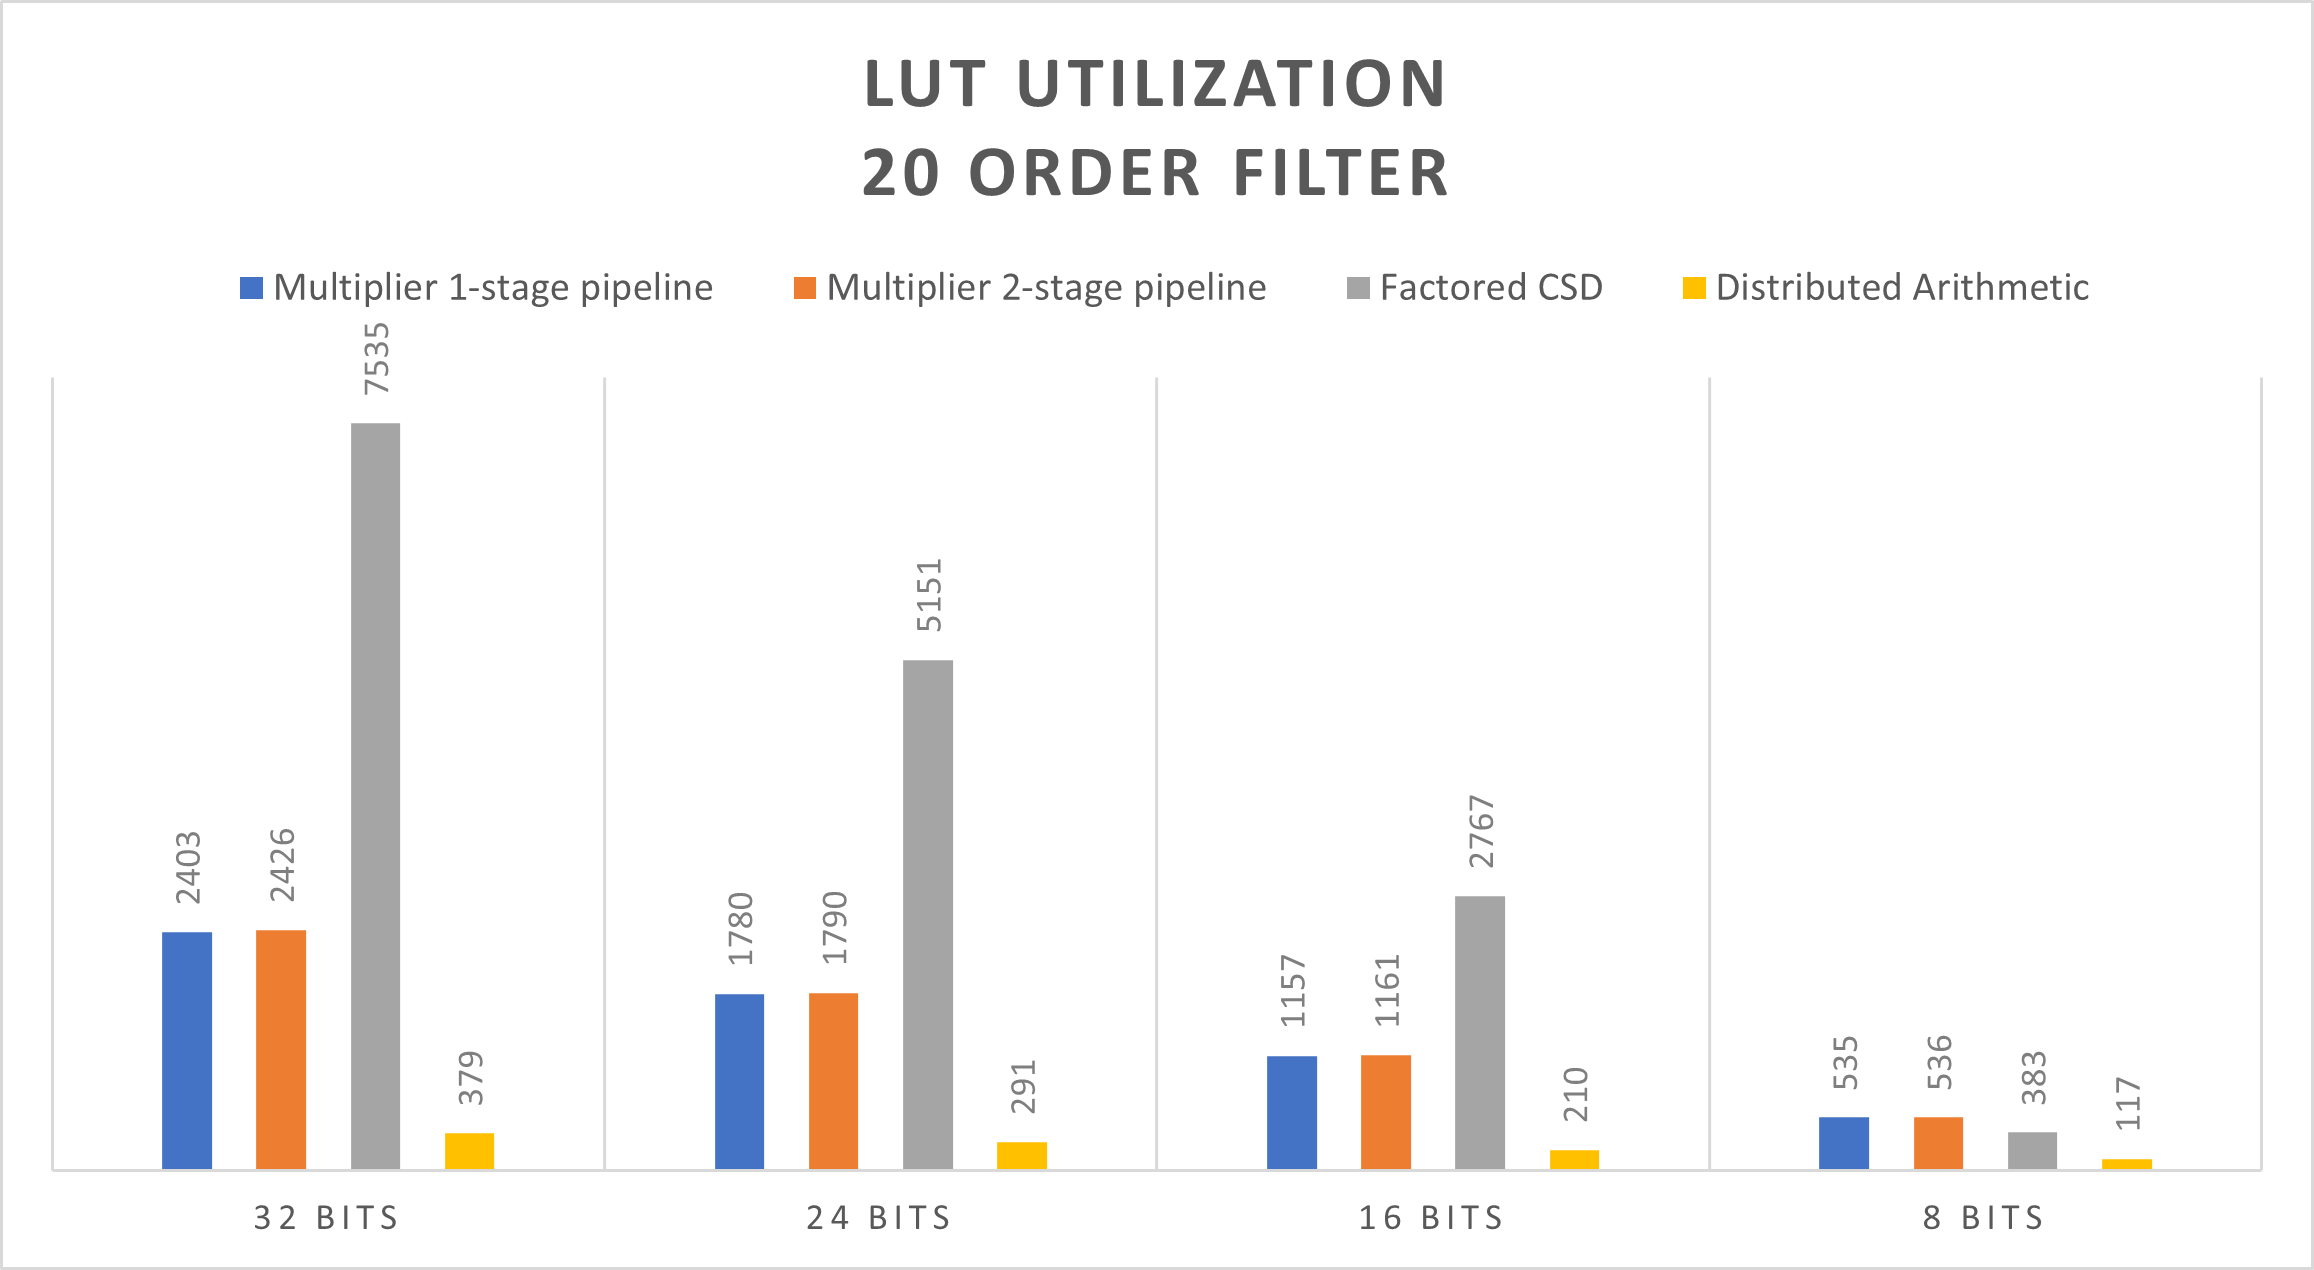
\includegraphics[width=0.45\textwidth]{../Images/FIR_20_Order/lut_utilization.png}
	}
	\subfigure[FF utilization of 30 order filter]{
		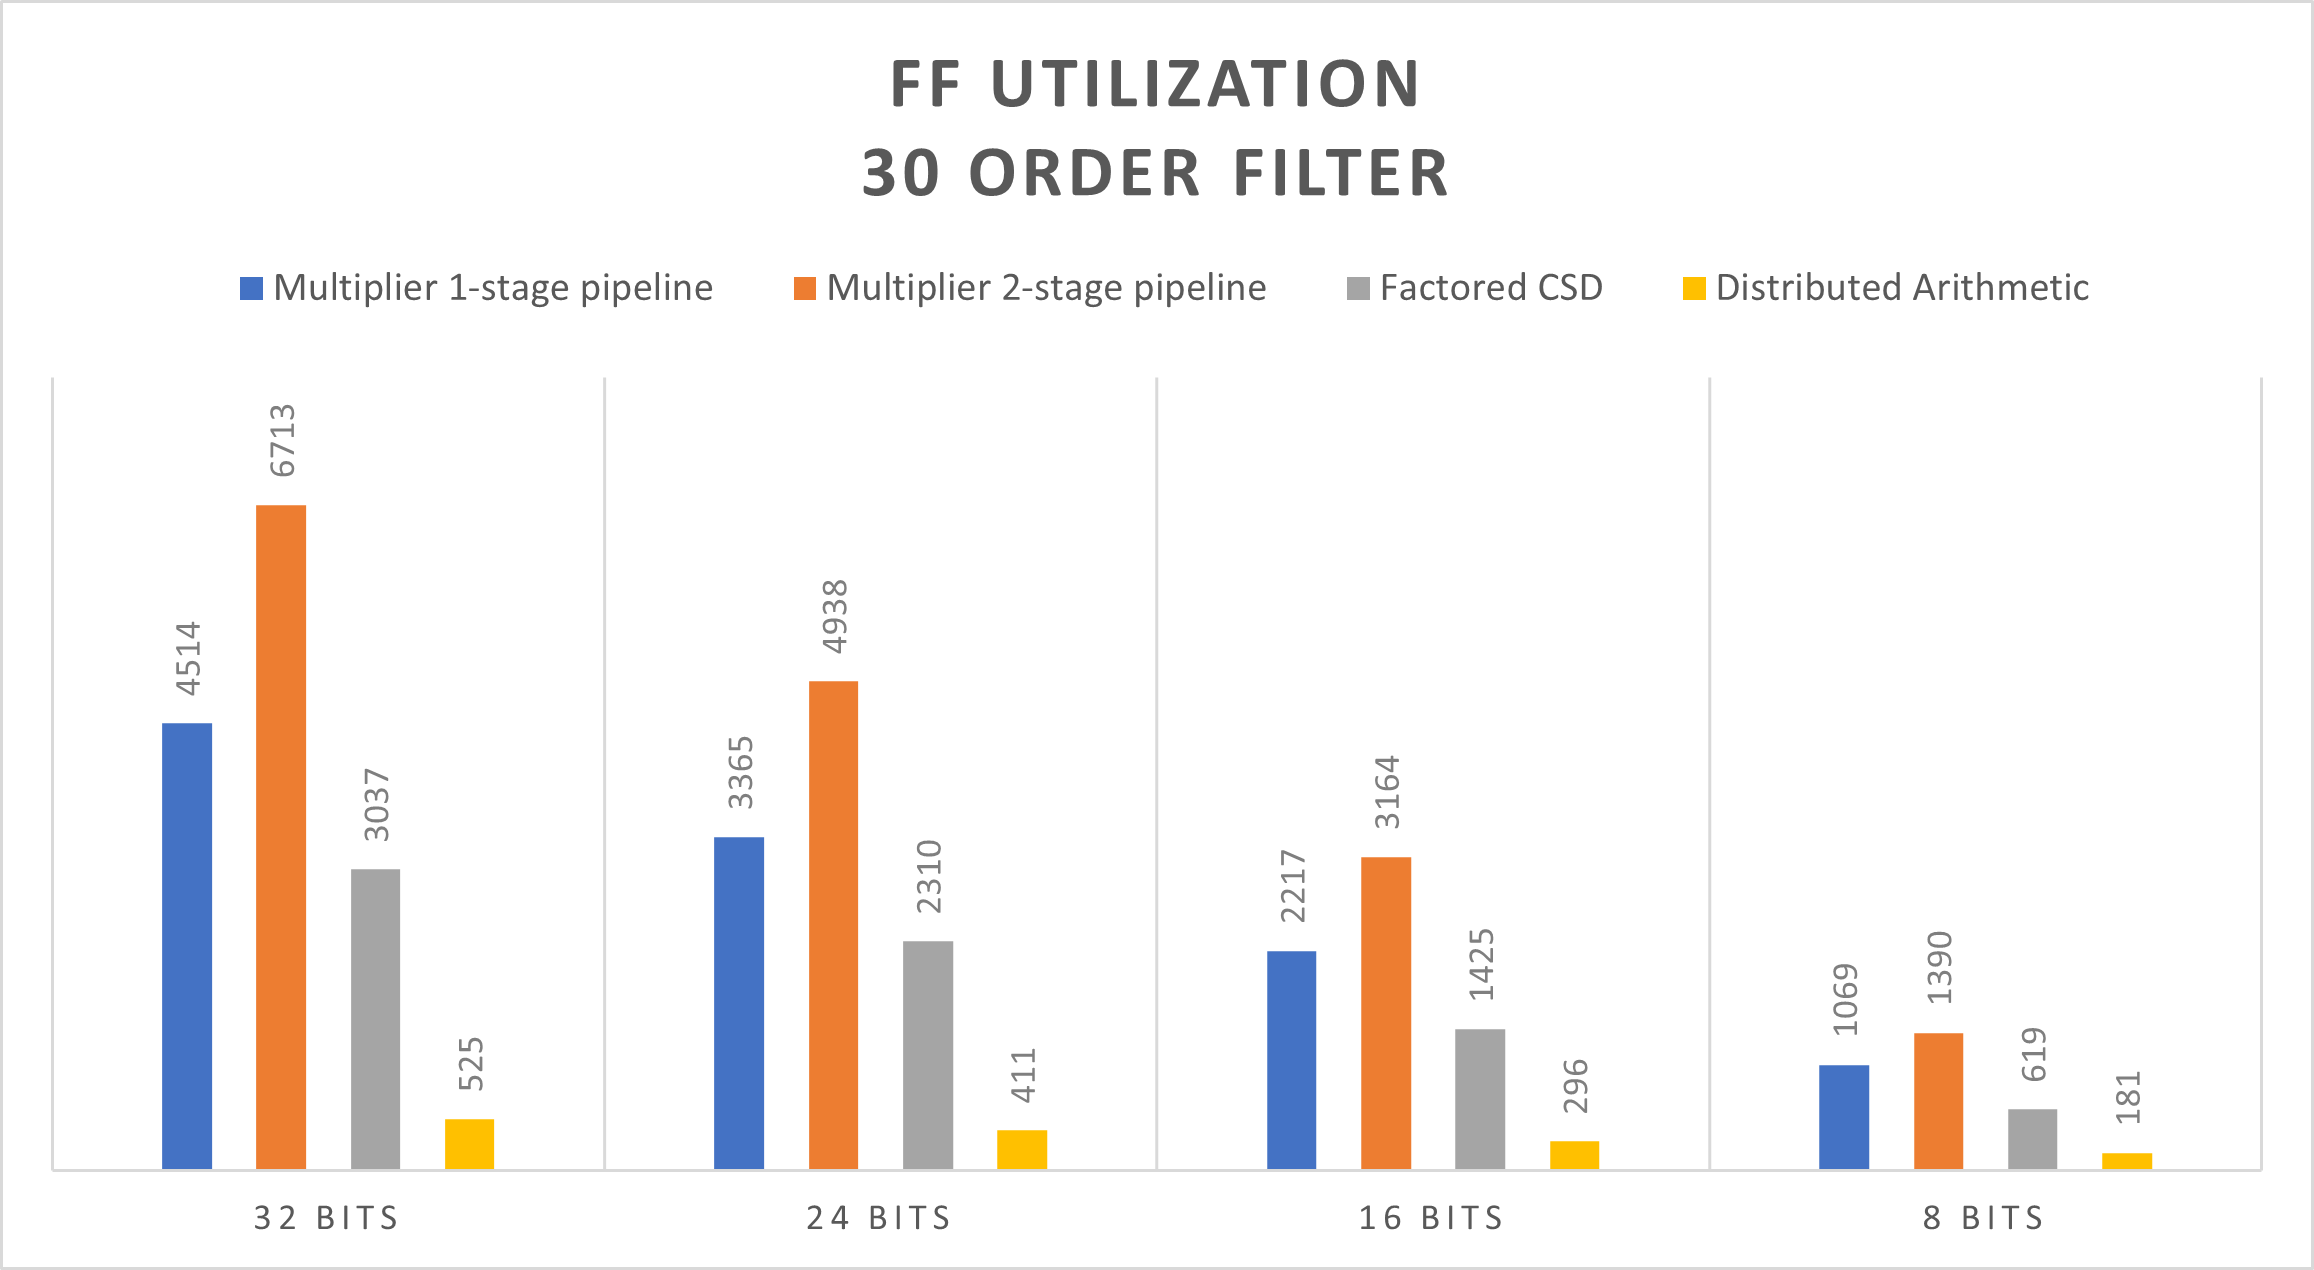
\includegraphics[width=0.45\textwidth]{../Images/FIR_30_Order/ff_utilization.png}
	}
	\subfigure[LUT utilization of min order filter]{
		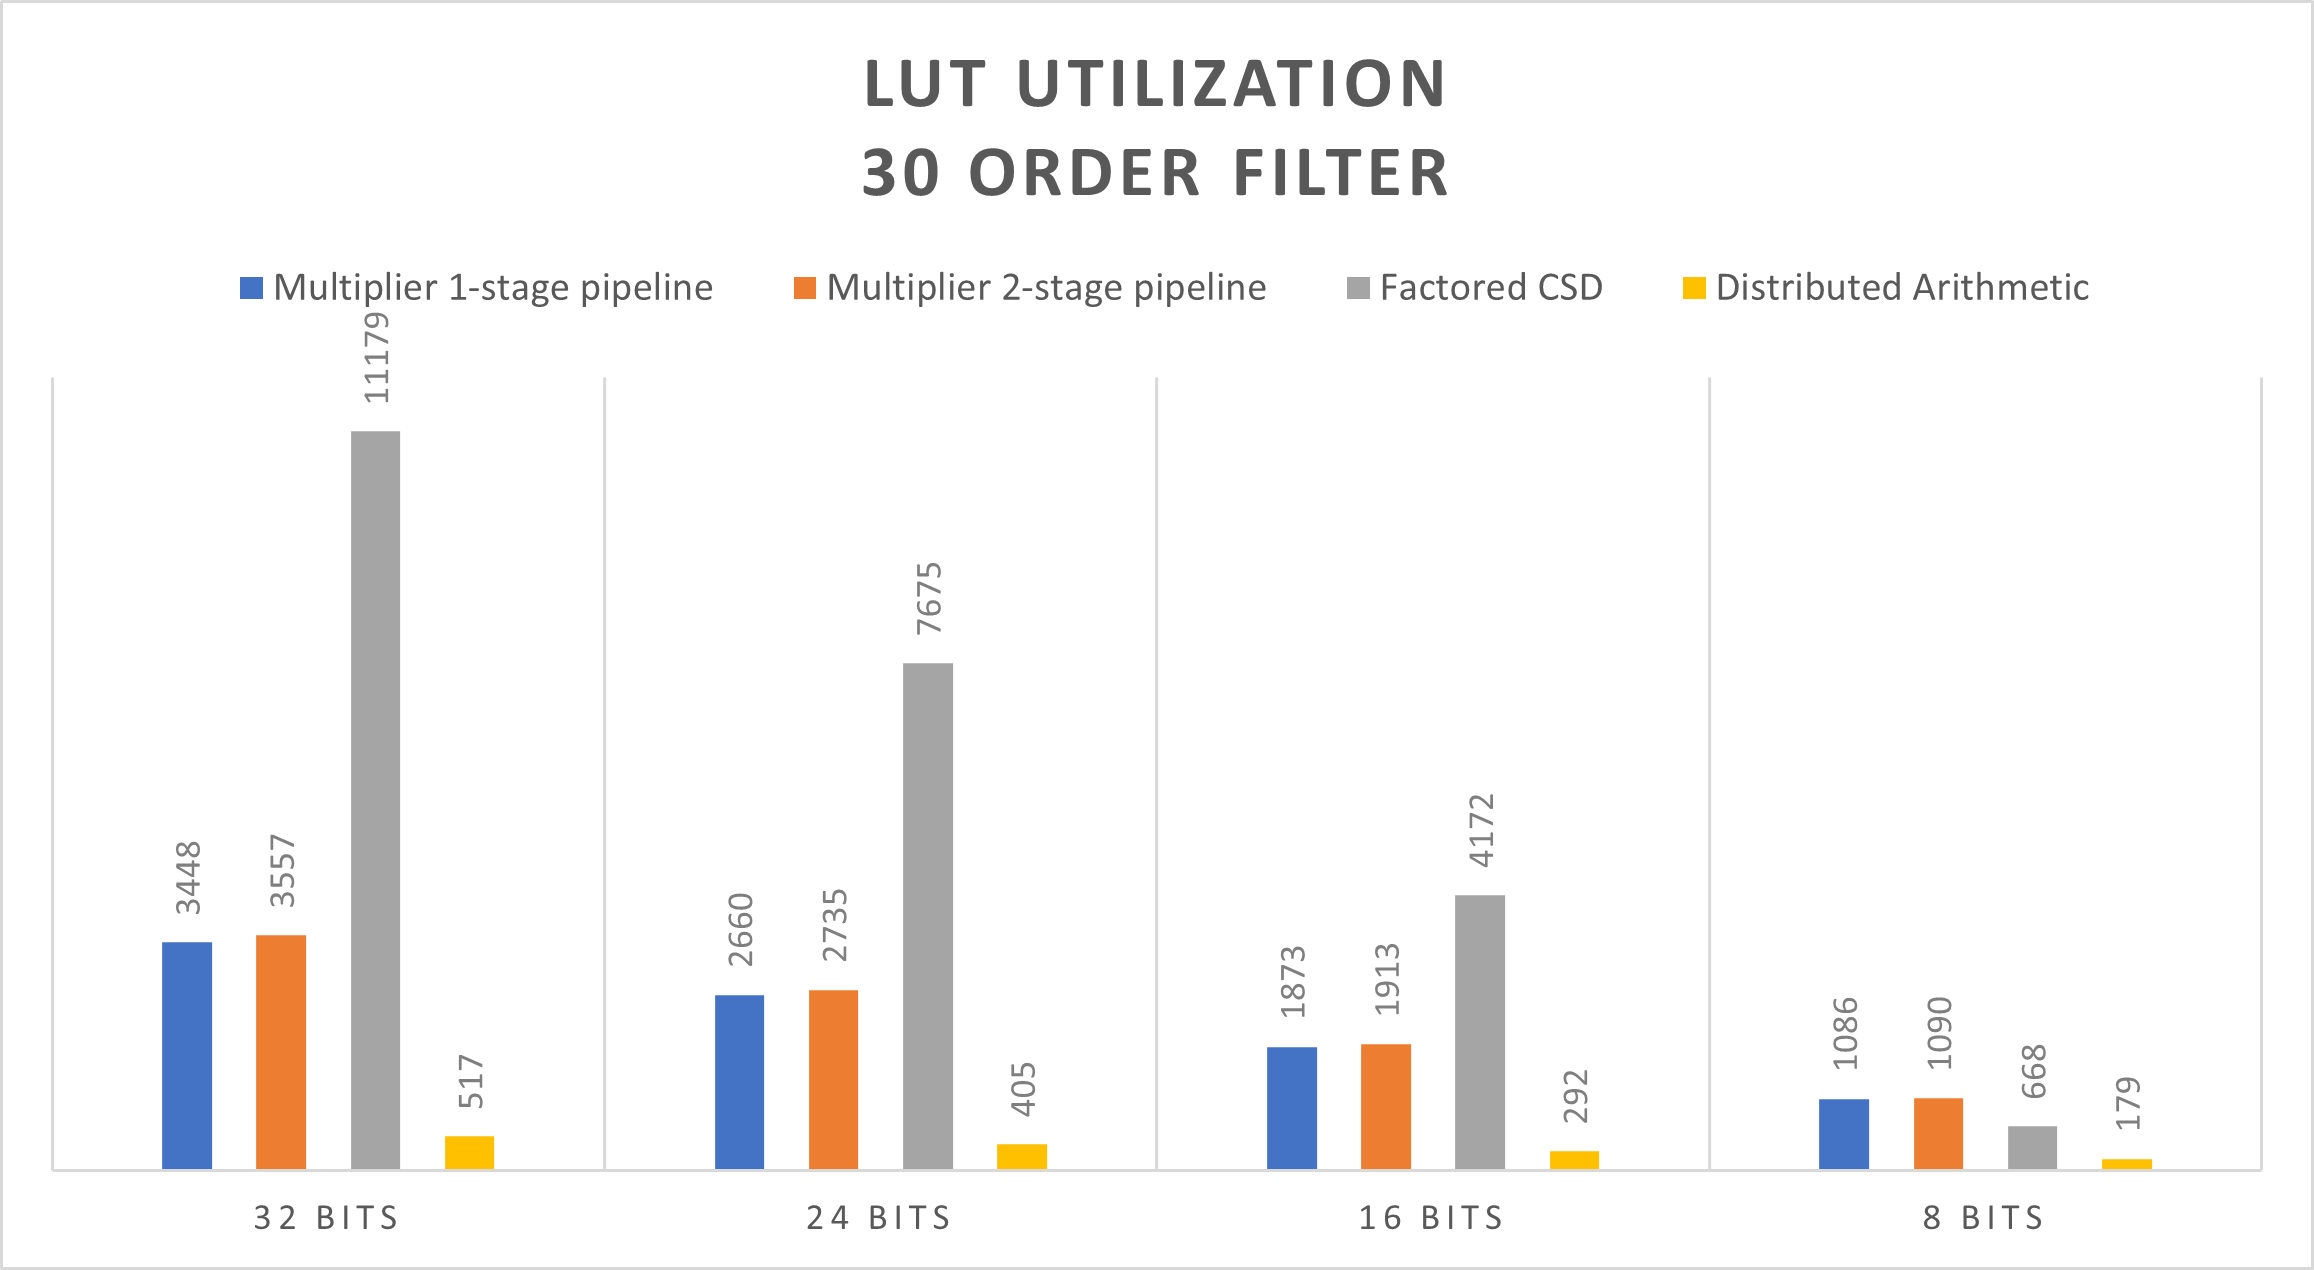
\includegraphics[width=0.45\textwidth]{../Images/FIR_30_Order/lut_utilization.png}
	}
	\caption{Various utilizations of LUTs and flip-flops for different architectures.}
	\label{fig:lut_ff_util_all}
\end{figure*}

